% -*- Mode:TeX -*-

%% IMPORTANT: The official thesis specifications are available at:
%%            http://libraries.mit.edu/archives/thesis-specs/
%%
%%            Please verify your thesis' formatting and copyright
%%            assignment before submission.  If you notice any
%%            discrepancies between these templates and the 
%%            MIT Libraries' specs, please let us know
%%            by e-mailing thesis@mit.edu

%% The documentclass options along with the pagestyle can be used to generate
%% a technical report, a draft copy, or a regular thesis.  You may need to
%% re-specify the pagestyle after you \include  cover.tex.  For more
%% information, see the first few lines of mitthesis.cls. 

%\documentclass[12pt,vi,twoside]{mitthesis}
%%
%%  If you want your thesis copyright to you instead of MIT, use the
%%  ``vi'' option, as above.
%%
%\documentclass[12pt,twoside,leftblank]{mitthesis}
%%
%% If you want blank pages before new chapters to be labelled ``This
%% Page Intentionally Left Blank'', use the ``leftblank'' option, as
%% above. 

\documentclass[12pt,twoside,singlespace]{mitthesis}
\usepackage{lgrind}
%% These have been added at the request of the MIT Libraries, because
%% some PDF conversions mess up the ligatures.  -LB, 1/22/2014
\usepackage{cmap}
\usepackage[T1]{fontenc}
\pagestyle{plain}
\usepackage[sort]{natbib}
\usepackage{algorithm}
\usepackage{algorithmic}
\usepackage{amsmath}
\usepackage{amsfonts}
\usepackage{graphicx}
\usepackage{paralist}
\usepackage{hyperref}
\usepackage{bm}
\usepackage{color}
\usepackage{tabularx}
\usepackage{subcaption}
\newcolumntype{Y}{>{\centering\arraybackslash}X}
%% This bit allows you to either specify only the files which you wish to
%% process, or `all' to process all files which you \include.
%% Krishna Sethuraman (1990).

%\typein [\files]{Enter file names to process, (chap1,chap2 ...), or `all' to
%process all files:}
%\def\all{all}
%\ifx\files\all \typeout{Including all files.} \else \typeout{Including only \files.} \includeonly{\files} \fi

\newcommand{\vr}[1]{\mbox{$\bm{#1}$}}
\newcommand{\vc}[1]{\mbox{\textbf{{$\mathsf #1$}}}}
\definecolor{RED}{rgb}{1.0,0.0,0.0}
\definecolor{BLACK}{rgb}{0.0,0.0,0.0}
\definecolor{WHITE}{rgb}{1.0,1.0,1.0}
\newcommand{\set}[1]{\mathcal{#1}}
\newcommand{\material}{\mathcal{M}}
\newcommand{\fe}{\mathcal{E}}
\newcommand{\note}[1]{#1}

\definecolor{DDFEMColor}{rgb}{0.49,0.49,0.8}
\definecolor{HiResColor}{rgb}{ 0.3686,0.5765 , 0.3961}
\definecolor{NaiveColor}{rgb}{ 0.6471, 0.3922, 0.4353}

\newcommand{\DDFEM}{{{\color{DDFEMColor}DDFEM}}}
\newcommand{\HiRes}{{{\color{HiResColor}High-Res Simulation}}}
\newcommand{\Naive}{{{\color{NaiveColor}Na\"{i}ve Coarsening}}}
\begin{document}

% -*-latex-*-
% 
% For questions, comments, concerns or complaints:
% thesis@mit.edu
% 
%
% $Log: cover.tex,v $
% Revision 1.8  2008/05/13 15:02:15  jdreed
% Degree month is June, not May.  Added note about prevdegrees.
% Arthur Smith's title updated
%
% Revision 1.7  2001/02/08 18:53:16  boojum
% changed some \newpages to \cleardoublepages
%
% Revision 1.6  1999/10/21 14:49:31  boojum
% changed comment referring to documentstyle
%
% Revision 1.5  1999/10/21 14:39:04  boojum
% *** empty log message ***
%
% Revision 1.4  1997/04/18  17:54:10  othomas
% added page numbers on abstract and cover, and made 1 abstract
% page the default rather than 2.  (anne hunter tells me this
% is the new institute standard.)
%
% Revision 1.4  1997/04/18  17:54:10  othomas
% added page numbers on abstract and cover, and made 1 abstract
% page the default rather than 2.  (anne hunter tells me this
% is the new institute standard.)
%
% Revision 1.3  93/05/17  17:06:29  starflt
% Added acknowledgements section (suggested by tompalka)
% 
% Revision 1.2  92/04/22  13:13:13  epeisach
% Fixes for 1991 course 6 requirements
% Phrase "and to grant others the right to do so" has been added to 
% permission clause
% Second copy of abstract is not counted as separate pages so numbering works
% out
% 
% Revision 1.1  92/04/22  13:08:20  epeisach

% NOTE:
% These templates make an effort to conform to the MIT Thesis specifications,
% however the specifications can change.  We recommend that you verify the
% layout of your title page with your thesis advisor and/or the MIT 
% Libraries before printing your final copy.
\title{Multiscale Methods for Design and Fabrication of Deformable Objects}

\author{Desai Chen}
% If you wish to list your previous degrees on the cover page, use the 
% previous degrees command:
%       \prevdegrees{A.A., Harvard University (1985)}
% You can use the \\ command to list multiple previous degrees
%       \prevdegrees{B.S., University of California (1978) \\
%                    S.M., Massachusetts Institute of Technology (1981)}
\department{Department of Electrical Engineering and Computer Science}

% If the thesis is for two degrees simultaneously, list them both
% separated by \and like this:
% \degree{Doctor of Philosophy \and Master of Science}
\degree{Doctor of Philosophy in Computer Science and Engineering}

% As of the 2007-08 academic year, valid degree months are September, 
% February, or June.  The default is June.
\degreemonth{September}
\degreeyear{2017}
\thesisdate{August 30, 2017}

%% By default, the thesis will be copyrighted to MIT.  If you need to copyright
%% the thesis to yourself, just specify the `vi' documentclass option.  If for
%% some reason you want to exactly specify the copyright notice text, you can
%% use the \copyrightnoticetext command.  
%\copyrightnoticetext{\copyright IBM, 1990.  Do not open till Xmas.}

% If there is more than one supervisor, use the \supervisor command
% once for each.
\supervisor{Wojciech Matusik}{Associate Professor}

% This is the department committee chairman, not the thesis committee
% chairman.  You should replace this with your Department's Committee
% Chairman.
\chairman{Mr. Chairman}{Chairman, Department Committee on Graduate Theses}

% Make the titlepage based on the above information.  If you need
% something special and can't use the standard form, you can specify
% the exact text of the titlepage yourself.  Put it in a titlepage
% environment and leave blank lines where you want vertical space.
% The spaces will be adjusted to fill the entire page.  The dotted
% lines for the signatures are made with the \signature command.
\maketitle

% The abstractpage environment sets up everything on the page except
% the text itself.  The title and other header material are put at the
% top of the page, and the supervisors are listed at the bottom.  A
% new page is begun both before and after.  Of course, an abstract may
% be more than one page itself.  If you need more control over the
% format of the page, you can use the abstract environment, which puts
% the word "Abstract" at the beginning and single spaces its text.

%% You can either \input (*not* \include) your abstract file, or you can put
%% the text of the abstract directly between the \begin{abstractpage} and
%% \end{abstractpage} commands.

% First copy: start a new page, and save the page number.
\cleardoublepage
% Uncomment the next line if you do NOT want a page number on your
% abstract and acknowledgments pages.
% \pagestyle{empty}
\setcounter{savepage}{\thepage}
\begin{abstractpage}
% $Log: abstract.tex,v $
% Revision 1.1  93/05/14  14:56:25  starflt
% Initial revision
% 
% Revision 1.1  90/05/04  10:41:01  lwvanels
% Initial revision
%
%% It will be single-spaced and the rest of the text that is supposed to go on
%% the abstract page will be generated by the abstractpage environment.  This
%% file should be \input (not \include 'd) from cover.tex.
Modern manufacturing technologies such as 3D printing enable the design and fabrication of objects with extraordinary complexity.
Arranging materials to form functional structures can achieve a much wider range of physical properties than in the constituent materials.
Many applications have been demonstrated in the fields of mechanics, acoustics, optics, and electromagnetics.
Unfortunately, it is difficult to design objects manually in the large combinatorial space of possible designs.
Computational design algorithms have been developed to automatically design objects with specified physical properties.
However, many types of physical properties are still very challenging to optimize because predictive and efficient simulations are not available for 
problems such as high-resolution non-linear elasticity or dynamics with friction and impact.
For simpler problems such as linear elasticity, where accurate simulation is available,
the simulation resolution handled by desktop workstations is still orders of magnitudes below available printing resolutions.

We propose to speed up simulation and inverse design process of fabricable objects by using multiscale methods.
First, we construct a library of microstructures and store their material properties such as Young's modulus and Poisson's ratio.
To use the library, the space of achievable material properties called the material property gamut is represented as a level set.
The level set enables efficient sampling of the gamut by focusing on finding samples near and outside the currently sampled boundary.
We use a combination of discrete and continuous sampling methods to push the structures to the limits of achievable material properties.
Next, with a pre-computed gamut, functional objects can be designed using microstructures instead of the base materials.
This allows us to simulate and optimize complex objects at a much coarser scale to improve simulation efficiency.
The speed improvement leads to the designs reaching a trillion voxels to match printer resolutions.
It also enables computational design of dynamic properties that can be faithfully reproduced in reality.
In addition to efficient design optimization, 
the gamut representation of the microstructure envelope provides a way to discover templates of microstructures with extremal physical properties.
In contrast to work where such templates are constructed by hand,
this is the first computational method to automatically discovery microstructure templates from voxel representations.

\end{abstractpage}

% Additional copy: start a new page, and reset the page number.  This way,
% the second copy of the abstract is not counted as separate pages.
% Uncomment the next 6 lines if you need two copies of the abstract
% page.
% \setcounter{page}{\thesavepage}
% \begin{abstractpage}
% % $Log: abstract.tex,v $
% Revision 1.1  93/05/14  14:56:25  starflt
% Initial revision
% 
% Revision 1.1  90/05/04  10:41:01  lwvanels
% Initial revision
%
%% It will be single-spaced and the rest of the text that is supposed to go on
%% the abstract page will be generated by the abstractpage environment.  This
%% file should be \input (not \include 'd) from cover.tex.
Modern manufacturing technologies such as 3D printing enable the design and fabrication of objects with extraordinary complexity.
Arranging materials to form functional structures can achieve a much wider range of physical properties than in the constituent materials.
Many applications have been demonstrated in the fields of mechanics, acoustics, optics, and electromagnetics.
Unfortunately, it is difficult to design objects manually in the large combinatorial space of possible designs.
Computational design algorithms have been developed to automatically design objects with specified physical properties.
However, many types of physical properties are still very challenging to optimize because predictive and efficient simulations are not available for 
problems such as high-resolution non-linear elasticity or dynamics with friction and impact.
For simpler problems such as linear elasticity, where accurate simulation is available,
the simulation resolution handled by desktop workstations is still orders of magnitudes below available printing resolutions.

We propose to speed up simulation and inverse design process of fabricable objects by using multiscale methods.
First, we construct a library of microstructures and store their material properties such as Young's modulus and Poisson's ratio.
To use the library, the space of achievable material properties called the material property gamut is represented as a level set.
The level set enables efficient sampling of the gamut by focusing on finding samples near and outside the currently sampled boundary.
We use a combination of discrete and continuous sampling methods to push the structures to the limits of achievable material properties.
Next, with a pre-computed gamut, functional objects can be designed using microstructures instead of the base materials.
This allows us to simulate and optimize complex objects at a much coarser scale to improve simulation efficiency.
The speed improvement leads to the designs reaching a trillion voxels to match printer resolutions.
It also enables computational design of dynamic properties that can be faithfully reproduced in reality.
In addition to efficient design optimization, 
the gamut representation of the microstructure envelope provides a way to discover templates of microstructures with extremal physical properties.
In contrast to work where such templates are constructed by hand,
this is the first computational method to automatically discovery microstructure templates from voxel representations.

% \end{abstractpage}

\cleardoublepage

\section*{Acknowledgments}

This is the acknowledgements section.  You should replace this with your
own acknowledgements.

%%%%%%%%%%%%%%%%%%%%%%%%%%%%%%%%%%%%%%%%%%%%%%%%%%%%%%%%%%%%%%%%%%%%%%
% -*-latex-*-

% Some departments (e.g. 5) require an additional signature page.  See
% signature.tex for more information and uncomment the following line if
% applicable.
% % -*- Mode:TeX -*-
%
% Some departments (e.g. Chemistry) require an additional cover page
% with signatures of the thesis committee.  Please check with your
% thesis advisor or other appropriate person to determine if such a 
% page is required for your thesis.  
%
% If you choose not to use the "titlepage" environment, a \newpage
% commands, and several \vspace{\fill} commands may be necessary to
% achieve the required spacing.  The \signature command is defined in
% the "mitthesis" class
%
% The following sample appears courtesy of Ben Kaduk <kaduk@mit.edu> and
% was used in his June 2012 doctoral thesis in Chemistry. 

\begin{titlepage}
\begin{large}
This doctoral thesis has been examined by a Committee of the Department
of Chemistry as follows:

\signature{Professor Jianshu Cao}{Chairman, Thesis Committee \\
   Professor of Chemistry}

\signature{Professor Troy Van Voorhis}{Thesis Supervisor \\
   Associate Professor of Chemistry}

\signature{Professor Robert W. Field}{Member, Thesis Committee \\
   Haslam and Dewey Professor of Chemistry}
\end{large}
\end{titlepage}


\pagestyle{plain}
  % -*- Mode:TeX -*-
%% This file simply contains the commands that actually generate the table of
%% contents and lists of figures and tables.  You can omit any or all of
%% these files by simply taking out the appropriate command.  For more
%% information on these files, see appendix C.3.3 of the LaTeX manual. 
\tableofcontents
\newpage
\listoffigures
\newpage
\listoftables


\chapter{Introduction}


\section{Motivations}


\section{Description}\label{ch1:desc}


\subsection{}


\subsection{}

\section{}


\subsection{}

\subsection{}

\section{}

\subsection{}

\subsection{}

\chapter{Data-Driven Coarsening of Finite Elements}
\section{Background}
\subsection{The Finite Element Method}
The finite element method~\citep{ciarlet2002finite} is a way to numerically approximate solutions to partial differential equations.
The function domain $\Omega$ is divided into a finite number of elements $E_k$.
A polynomial function is defined over each element.
These polynomials form a basis for finite-dimensional approximations to the solution.

This thesis uses the eight-node hexahedron element defined in $\mathbb{R}^3$
to perform all of the mechanical analysis.
The eight-node hexahedron element is the simplest of the hexahedron family.
It represents continuous functions supported inside the element by trilinearly interpolating function values defined on its eight nodes.
Each node $\mathbf{X}_i$ resides in $\mathbb{R}^3$ with a given real value $u(\mathbf{X}_i)$.
The nodal positions must cooperate to guarantee that no point inside the hexahedron is inverted.
This will be explained later.
For now, suppose the element shape is well-defined and 
consider a point $\mathbf{X}\in\mathbb{R}^3$ inside the element.
The trilinear interpolation on $\mathbf{X}$ is given by
\[
u(\mathbf{X})=\sum_i N_iu(\mathbf{X}_i),
\]
for some weights $N_i$ that depends on the relative position between $\mathbf{X}$ 
and $\mathbf{X}_i$. These weighting functions are called \textbf{shape functions}.

In order to write down the expression for $N_i$, we need to introduce the standard quadrilateral or hexahedral element (Figure~\ref{fig:standardEle}).
The standard hexahedron is just a cube centered at the origin spanning $[-1,1]^3$.
The axis are labeled with $\xi, \eta, \zeta$ to distinguish from the space that $\mathbf{X}$ resides in.
This new coordinate system is known as the isoparametric hexahedral coordinates or more commonly referred to as \textbf{natural coordinates}.
The nodal positions of the standard elements in the natural coordinates are listed in Table~\ref{tab:natCoord}.
For a point $\chi=(\xi, \eta,\zeta)$ in the natural coordinates,
its interpolation weights is defined as in Equation~\ref{eq:triWeight}.
\begin{equation}
	N_i(\chi)=\frac{1}{8}(1+\xi_i\xi)(1+\eta_i\eta)(1+\zeta_i\zeta).
	\label{eq:triWeight}
\end{equation}
Note that the sum of the weights is always $1$ for any point inside the element.
Suppose now we define a ``density'' value of $1$ on each of its eight vertices,
we can compute the total mass of the element by 
\[
mass=\int_{-1}^{1}\int_{-1}^{1}\int_{-1}^{1}\sum_i w_i\cdot 1 \,d\xi \,d\eta\,d\zeta=
\int_{-1}^{1}\int_{-1}^{1}\int_{-1}^{1} 1 \,d\xi \,d\eta\,d\zeta=8.
\]
This is simply the volume of the standard element multiplied by the density.
This partition of unity property of the interpolation function is crucial for physical meanings of quantities defined on the element.
\begin{figure}
\centering
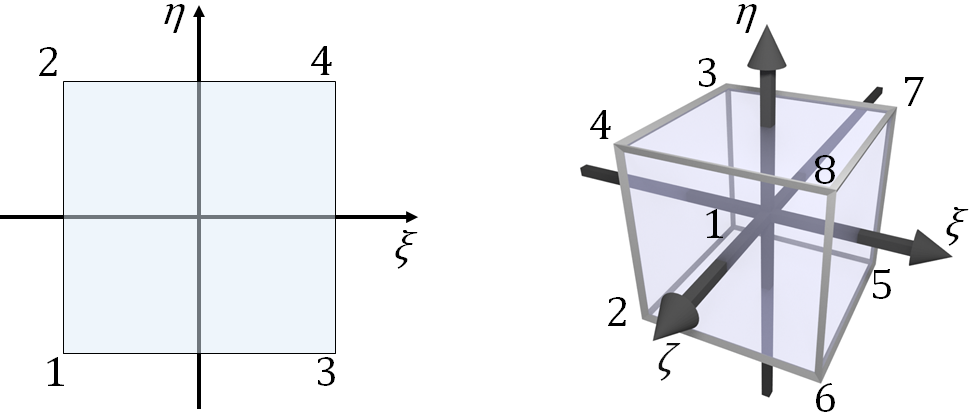
\includegraphics[width=0.8\textwidth]{figs/refEle.png}
\caption{Standard elements for 2D quadrilateral (left) 
	and 3D hexahedral elements (right). The standard element spans $[-1,1]$ in each axis
	to facilitate Gaussian quadrature rules. Nodes are marked with their indices.
	}
\label{fig:standardEle}
\end{figure}
\begin{table}
	\begin{center}
		\begin{tabular}{ |c| r r r|}
			\hline
			Index & $\xi_i$ & $\eta_i$ & $\zeta_i$ \\ \hline
			1 & -1 & -1 & -1\\  
			2 & -1 & -1 & 1\\
			3 & -1 & 1 & -1\\  
			4 & -1 & 1 & 1\\
			5 & 1 & -1 & -1\\  
			6 & 1 & -1 & 1\\
			7 & 1 & 1 & -1\\  
			8 & 1 & 1 & 1\\
		\hline						
		\end{tabular}
	\end{center}
	\caption{Nodal positions of the standard hexahedron element in the natural coordinates.
		Coincidentally, these coordinate values can also be used to define the trilinear interpolation weights.}
	\label{tab:natCoord}
\end{table}

With the interpolation function fully defined in the natural coordinates, 
we can use it to map a point $\chi$ in natural coordinates to a point
$\mathbf{X}$ inside a general hexahedron element with nodal positions $\mathbf{X}_i$ as follows
\begin{equation}
	\mathbf{X}=\sum_i N_i(\chi)\mathbf{X}_i.
	\label{eq:rest}
\end{equation}

Note here we are interpolating a vector-valued function where each coordinate is interpolated independently.
\subsection{Modeling Elastic Objects}
Elastic objects tend to return to its rest shape when deformed by external forces such as stretching, bending, twisting etc. The direction and strength of the tendency to restore to its rest shape is described by its elastic forces.
To model the exact behavior of a small piece of material,
we first use finite elements to approximate its deformations.
A hexahedron element models a piece of elastic material that can deform by changing its nodal positions.
The internal volume deforms by following the nodal displacements using trilinear interpolation.
Of course real materials do not have to deform this way.
The trilinear interpolation is only an approximation.
More precisely, for an element with a rest configuration given by $\mathbf{X}_i$,
its nodes can be moved to new positions $\mathbf{x}_i$ by displacements $\mathbf{u}_i$,
i.e., $\mathbf{x}_i=\mathbf{X}_i+\mathbf{u}_i$.
For any point $\mathbf{X}$ inside the element with known natural coordinates $\chi$, its displacement $\mathbf{u}(\mathbf{X})$ is given by interpolation
\begin{equation}
\mathbf{u}(\mathbf{X}) = \sum_iN_i(\chi)\mathbf{u}_i.
\label{eq:disp}
\end{equation}
To make a clear distinction between $\mathbf{X}$ and $\mathbf{x}$,
$\mathbf{X}$ is defined as a point in the \textbf{reference space} that represents the undeformed shape of an object. The lower case $\mathbf{x}$ lives in the \textbf{deformed space} that represents the deformed configuration of an object.

From now on, to simplify notation, $N_i(\xi)$ will be written as $N_i$.
The deformation of an object is quantified using strain measures,
which is defined in terms of the difference in displacement between nearby points.
Intuitively, if $\mathbf{u}(\mathbf{X})$ is constant, then the displacement field is just a translation. In this case the material is undeformed and should not contain any strain.
More generally, the difference of displacement between nearby points can be written using derivatives,
\[
\mathbf{F}=\frac{\partial \mathbf{u}}{\partial \mathbf{X}}+\mathbf{I}
=\begin{pmatrix}
\dfrac{\partial u_1}{\partial X_1} & \dfrac{\partial u_1}{\partial X_2}&\dfrac{\partial u_1}{\partial X_3}\\
\dfrac{\partial u_2}{\partial X_1} & \dfrac{\partial u_2}{\partial X_2}&\dfrac{\partial u_2}{\partial X_3}\\
\dfrac{\partial u_3}{\partial X_1} & \dfrac{\partial u_3}{\partial X_2}&\dfrac{\partial u_3}{\partial X_3}\\
\end{pmatrix}+\mathbf{I}.
\]
The matrix $\mathbf{F}$ is the \textbf{deformation gradient} and $\mathbf{I}$ is the identity matrix.
While we do not have a closed-form expression of $\mathbf{u}$ written in terms of $\mathbf{X}$,
we have Equation~\ref{eq:rest} and~\ref{eq:disp} that relate $\mathbf{u}$ and $\mathbf{X}$ through $\chi$.
The term $\frac{\partial \mathbf{u}}{\partial \mathbf{X}}$ can be re-written using the chain rule,
\begin{equation}
\frac{\partial \mathbf{u}}{\partial \mathbf{X}}=
\frac{\partial \mathbf{u}}{\partial \chi}
\frac{\partial \chi}{\partial \mathbf{X}}=
(\sum_i\mathbf{u}_i\frac{dN_i}{d\chi})(\frac{\partial \mathbf{X}}{\partial \chi})^{-1}
\label{eq:dudX}
\end{equation}
The matrix $\frac{\partial \mathbf{X}}{\partial \chi}$ is called the Jacobian matrix of $\mathbf{X}$ with respect to $\chi$ and is written as
\[
\mathbf{J}=\frac{\partial \mathbf{X}}{\partial \chi}
= \sum_i\mathbf{X}_i\frac{dN_i}{d\chi}.
\]
By convention, $\frac{dN_i}{d\chi}$ is a $1\times 3$ row vector.
The term $\mathbf{X}_i\frac{dN_i}{d\chi}$ is an outer product that produces a $3\times 3$ matrix.

Given the full expression for the deformation gradient $\mathbf{F}$, we can now define elastic energy densities. 
The elastic energy density function $\Psi(\mathbf{F})$ computes a non-negative energy value given a deformation gradient.
This function fully defines the elastic behavior of a piece of material especially the elastic forces.
Integrating $\Psi$ over the domain $\Omega$ of an element in the reference space yields the total elastic energy contained by that element.
\[
E(\mathbf{x}_1,...,\mathbf{x}_8)=\int_{\Omega}\Psi dV.
\]
Differentiating $E$ with respect to nodal positions $\mathbf{x}_i$ gives us the opposite direction of nodal elastic forces
\[
-\mathbf{f}_i=\frac{dE}{d\mathbf{x}_i}=\int_{\Omega}
\frac{d\Psi(\mathbf{F})}{d\mathbf{F}}
\frac{d\mathbf{F}}{d\mathbf{x}_i}dV
=\int_{\Omega}
\mathbf{P}(\mathbf{F})
\frac{d\mathbf{F}}{d\mathbf{x}_i}dV,
\]
Where
\[
\mathbf{P}(\mathbf{F})=\dfrac{d\Psi(\mathbf{F})}{d\mathbf{F}}.
\]
$\mathbf{P}(\mathbf{F})$ is called the fist Piola-Kirchhoff stress.
It transforms a normal vector in the reference space to a force acting in the deformed configuration divided by area in the reference space.
Integrating in the reference space is not easy since the element is not necessarily a rectangular shape. By change of variables, we can integrate in natural coordinates
in the set $\Omega_{\chi}=[-1,1]^3$.
\begin{align*}
\int_{\Omega}
\mathbf{P}(\mathbf{F})
\frac{d\mathbf{F}}{d\mathbf{x}_i}dV
&=\int_{\Omega_{\chi}}
\mathbf{P}(\mathbf{F})
\frac{d\mathbf{F}}{d\mathbf{x}_i}|\det{\mathbf{J}}|dV\\
&=\int_{\Omega_{\chi}}
\mathbf{P}(\mathbf{F})\mathbf{J}^{-T}
\frac{dN_i}{d\chi}\det{\mathbf{J}}\,dV.
\end{align*}
Here we dropped the absolute value sign because the undeformed element is required to have positive determinant everywhere.
To numerically evaluate the integral, we use Gaussian quadrature rules.
For example, the two-point Gaussian quadrature rule places quadrature points at
$\pm \sqrt{\frac{1}{3}}$ in natural coordinates, which results in $8$ quadrature points with equal weights in 3D.
For each quadrature point $j$, we evaluate the integrand and multiply by the quadrature weight $w_j$. The integral is written as a summation
\[
-\mathbf{f}_i=\sum_j w_j\mathbf{P(\mathbf{F}_j)}\mathbf{J}^{-T}
\frac{dN_i}{d\chi}\det{\mathbf{J}}.
\]

$\Psi$ determines the constitutive model of elasticity, i.e. the relationship between strain measures and stress.
This thesis primarily uses two kinds of constitutive models: linear elasticity and Neo-Hookean model. For the linear elasticity, we first define the infinitesimal strain tensor
\[
\epsilon = \frac{1}{2}(\mathbf{F}+\mathbf{F}^T)-I.
\]
This strain tensor is a symmetric matrix. The stress tensor derived from this strain measure is also a symmetric matrix. This property is a necessary condition for conservation of linear and angular momentum. 
In other words, stress and internal elastic forces should not cause any change in total linear or angular momentum.
The strain energy density function for isotropic linear elasticity is
\[
\Psi(\mathbf{F}) = \mu\epsilon:\epsilon + \frac{\lambda}{2}tr^2(\epsilon).
\]
$\mu$ is a material parameter called shear modulus and $\lambda$ is Lam\'{e}'s first parameter.
$tr(\epsilon)$ is the trace of the strain tensor.
Differentiate $\Psi$ to obtain
\[
\mathbf{P}(\mathbf{F})=\mu(\mathbf{F}+\mathbf{F}^T-2\mathbf{I})+\lambda tr(\mathbf{F}-\mathbf{I})\mathbf{I}.
\]
For anisotropic linear elasticity, the constitutive equation is written as
\begin{equation}
\sigma=\mathbf{C}\epsilon,
\label{eq:constitutive}
\end{equation}
where $\sigma$ is the $3\times 3$ Cauchy stress tensor, $\mathbf{C}$ is a
fourth-order $3\times 3\times3\times3$ tensor called the tensor of elasticity.
The term $\mathbf{C}\epsilon$ is a summation of component-wise products.
In Einstein notation,
\[
\sigma_{ij}=C_{ijkl}\epsilon_{kl}.
\]
Cauchy stress relates to the first Piola-Kirchhoff stress by
\[
\sigma = \frac{1}{\det \mathbf{F}}\mathbf{P}\mathbf{F}^T
\]
The corresponding strain energy density function is
\[
\Psi(\epsilon)=\frac{1}{2}\mathbf{C}\epsilon^2.
\]
To simplify notations, the stress and strain tensors are written as vectors instead of matrices.
Using Voigt notation,
a stress tensor of the form
\[
\sigma=\begin{pmatrix}
\sigma_{xx} & \sigma_{xy} & \sigma_{xz}\\
\sigma_{yx} & \sigma_{yy} & \sigma_{yz}\\
\sigma_{zx} & \sigma_{zy} & \sigma_{zz}
\end{pmatrix}
\]
is rewritten as
\[\sigma=(\sigma_{xx} , \sigma_{yy} , \sigma_{zz},
\sigma_{xy} , \sigma_{yz} , \sigma_{zx}).
\]
This allows the tensor of elasticity to be written as a $6\times 6$ matrix.
For orthotropic linear materials, $\mathbf{C}$ takes the following form
\[
\mathbf{C}=
\begin{pmatrix}
C_{1111} & C_{1122} & C_{1133} & 0 & 0 & 0 \\
 & C_{2222} & C_{2233} & 0 & 0 & 0 \\
& & C_{3333} & 0 & 0 & 0 \\
& & & C_{1212} & 0 & 0 \\
 & Symm &  & & C_{2323} & 0 \\
 & & & & & C_{1313}
\end{pmatrix}.
\]
For a more restricted subset of materials with cubic symmetry, 
$\mathbf{C}$ is specified by three material parameters: Young's modulus $E$,
Poisson's ratio $\nu$, and shear modulus $G$ or $\mu$.
\[\mathbf{C}=
\begin{pmatrix}
(1-\nu)\hat{E} & \nu\hat{E} & \nu\hat{E} & 0 & 0 & 0 \\
&(1-\nu)\hat{E} & \nu\hat{E} & 0 & 0 & 0 \\
& &(1-\nu)\hat{E} & 0 & 0 & 0 \\
& & & \mu & 0 & 0 \\
& Symm &  & & \mu & 0 \\
& & & & & \mu
\end{pmatrix},\hat{E} = \frac{E}{(1-2\nu)(1+\nu)}.
\]

The advantage of the linear elasticity is that it assumes a linear relationship between stress and strain. This leads to a linear relationship between nodal displacements and nodal forces
as follows
\[
\mathbf{K}\mathbf{U}=-\mathbf{f}.
\]
Here $\mathbf{K}$ is called the stiffness matrix given by
\[
\mathbf{K}=\frac{\partial^2 \Psi}{\partial\mathbf{U}^2}.
\]
$\mathbf{U}$ is the concatenated nodal displacement vector
$[\mathbf{u}_1,\mathbf{u}_2,...,\mathbf{u}_8]$ and $\mathbf{f}$ is the concatenated internal nodal force vector.
Computing the deformation under external boundary conditions and forces requires only a single linear solve
\[
\mathbf{U}=\mathbf{K}^{-1}\mathbf{f}_{ext},
\]
given sufficient boundary conditions.
The stiffness matrix is sparse and positive semi-definite (positive definite with enough constraints).
A wide class of linear solvers have been developed for such linear systems.
To see the linear relationship between displacements and force,
we just need to derive the linear relationship between $\epsilon$ and $\mathbf{u}_i$
from Equation~\ref{eq:dudX} and combine it with Equation~\ref{eq:constitutive}.
For a point $\mathbf{X}\in\mathbb{R}^3$, we will use superscripts to denote its individual coordinates.
Define the strain-displacement matrix
\[
\mathbf{B}(\mathbf{X})=
\begin{pmatrix}
\dfrac{dN_1}{d\mathbf{X}^1} & 0 & 0 & ... \\
0 & \dfrac{dN_1}{d\mathbf{X}^2} & 0 & ... \\
0 & 0 & \dfrac{dN_1}{d\mathbf{X}^3} & ... \\
\dfrac{dN_1}{d\mathbf{X}^2} & \dfrac{dN_1}{d\mathbf{X}^1} & 0 & ... \\
0 & \dfrac{dN_1}{d\mathbf{X}^3} & \dfrac{dN_1}{d\mathbf{X}^2} & ... \\
\dfrac{dN_1}{d\mathbf{X}^3} & 0 & \dfrac{dN_1}{d\mathbf{X}^1} & ...
\end{pmatrix}.
\]
For an eight-node hexahedron, this matrix has $3\times 8=24$ columns.
This matrix computes the strain tensor at a point $\mathbf{X}$ given nodal displacements
\[
\epsilon(\mathbf{X})=\mathbf{B}(\mathbf{X})\mathbf{U}.
\]
This linear relationship concludes our claim that linear elasticity model defines a linear relationship between nodal displacements and nodal forces.
Further, using quadrature rules, we can numerically evaluate $\mathbf{K}$ as
\[
\mathbf{K}=\sum_j w_j \mathbf{B}(\mathbf{X}_j)\mathbf{C}\mathbf{B}(\mathbf{X}_j)\det \mathbf{J}.
\]

The downside of linear elasticity is that it does not handle rotation properly.
An elastic object undergoing a rigid rotation should contain zero elastic energy.
If we let $\mathbf{F}=\mathbf{R}$ for some rotation matrix $\mathbf{R}$,
the resulting energy measure is generally non-zero.
This constitutive model is useful only when the deformation is small with respect to the overall size of the object.
When an object undergoes buckling with many potential static equilibrium configurations,
linear elasticity always predict a single solution with little buckling since its elastic energy landscape is convex with a unique local minimum.
Additionally, linear elasticity does not preserve volume according to the Poisson's ratio parameter. In fact, elements can easily invert into non-physical states.

To address the rotation problem, non-linear elasticity models such as the corotated linear elasticity model and the Saint-Venant Kirchhoff model are developed to be rotation invariant.
However, these models still allow an element to invert and do not preserve volume.
We use the Neo-Hookean material model for non-linear elasticity. It resists inverting, and approximately preserves volume according to Poisson's ratio.
The strain energy density of Neo-Hookean model is
\[
\Psi(\mathbf{F})=\frac{\mu}{2}(I_1-3) - \mu \log \det \mathbf{F} 
+ \frac{\lambda}{2}(\log \det \mathbf{F})^2,
\]
where the first isotropic invariant is 
\[
I_1=tr(\mathbf{F}^T\mathbf{F}).
\]
The first Piola-Kirchhoff stress is
\[
\mathbf{P}(\mathbf{F})=\mu(\mathbf{F}-\mathbf{F}^{-T})+\lambda(\log\det\mathbf{F})\mathbf{F}^{-T}.
\]
\section{Data-Driven Coarsening}
Objects with high-resolution, heterogeneous elastic materials are everywhere:
from the output of multimaterial 3D printers to virtual characters 
gracing the screen in our summer blockbusters.
Designing such objects is made possible by the tight coupling of design
tools and numerical simulation which allows designers or automatic
algorithms to update geometry or material parameters and subsequently
estimate the physical effects of the change.
Fast, accurate simulation techniques that can handle runtime changes in geometry
and material composition are a necessity for such iterative design algorithms.
There have been a large number of works on speeding up FEM simulations,
and these speed improvements have enabled FEM to be used in many performance critical tasks 
such as computer animation, surgical training, and virtual/augmented reality.
Even though techniques such as model reduction or numerical coarsening can
achieve order-of-magnitude performance increases,
they require expensive precomputation phases, typically on the order of minutes for large meshes.
This precomputation requires knowledge of an
object’s geometry and material composition a priori, something
that is not known during a design task.
When the user updates the model by changing the geometry or the material distribution,
the preprocessing step must be run again.
As shown in Figure~\ref{fig:typical}a, since this step is inside the design loop,
the user cannot get rapid feedback on the changes made to the object.
\begin{figure}
	\centering
	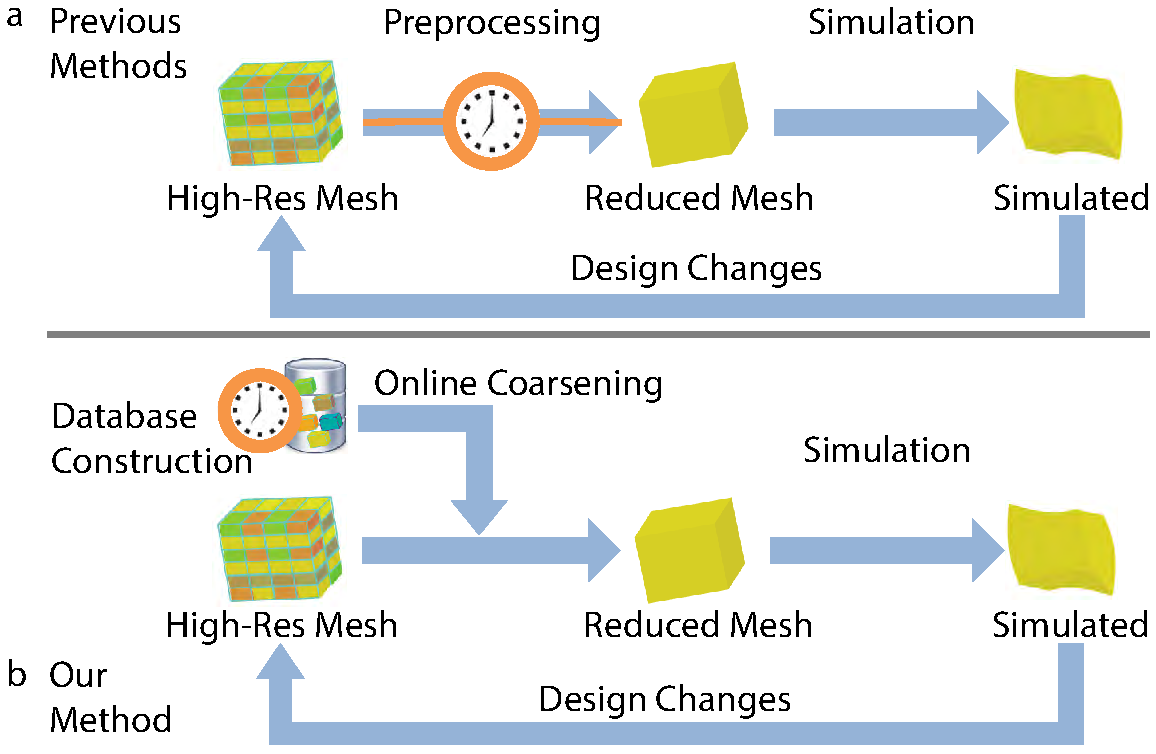
\includegraphics[width=0.8\textwidth]{figs/typical1.pdf}
	\caption{(a) In a typical method, the preprocessing step is offline,
		making the design loop slow. (b) In our method, we move the timeconsuming
		offline computation outside of the design loop.}
	\label{fig:typical}
\end{figure}

We propose Data-Driven FEM (DDFEM), a new simulation methodology
that removes these limitations and is thus extremely well suited
to the types of design problems discussed above.
We divide an object into a set of deformable voxels using embedded finite
elements and coarsen these voxels hierarchically.
A custom metamaterial database is populated with materials that minimize the error incurred by coarsening.
This database is learned once in a completely offline fashion and depends only on the set of materials to be used by the deformable object and not on the actual material distribution
and geometry.
At runtime we use the database to perform fast coarsening of an FEM mesh in a way that is agnostic to changes in geometry and material composition of the object.
The key features of the algorithm are its ability to handle arbitrary, nonlinear elastic
constitutive models as well as to avoid expensive precomputation
within the design loop (Figure~\ref{fig:typical}b).
DDFEM is the first algorithm optimized for interactive design of non-linear elastic objects.

DDFEM is a combination of embedded finite elements and hierarchical
coarsening.
In the remainder of this section, we discuss the problem of coarsening
and introduce the notion of a material palette. We conclude by
summarizing the two main stages of DDFEM—offline coarse material
construction and online coarsening.
\paragraph{Coarsening for finite elements}
The key component of our DDFEM is coarsening.
Coarsening reduces the number of vertices in a finite element simulation mesh in order to improve
runtime performance.
Since simply removing vertices can greatly reduce
the accuracy of the simulation, coarsening schemes also assign
new materials to coarsened elements to minimize this effect.
We regard the global coarsening of a simulation mesh as the result
of many local coarsening operations which map from contiguous
subsets of fine elements with applied materials to coarse elements
with new, optimized materials. Our goal is to precompute these
optimized materials so that coarsening is fast at runtime. Below we
discuss how to make such a precomputation tractable beginning with
our choice of finite element simulation methodology.
\paragraph{Conforming vs. embedded finite elements}
The defining feature of conforming finite element methods is that the simulation
mesh is aligned with the geometry of the object being simulated.
One obvious feature of conforming meshes is that the mesh itself is a
function of the input geometry.
This means that the output of a local coarsening operator (the coarsened mesh) will also be a function
of the input geometry.
Also, the new material computed by each local coarsening operator will be a function of input geometry.
This dependence on input geometry is a significant issue to overcome
if we wish to precompute coarsened materials because, in design
problems, the input geometry is in constant flux.
The number of precomputed coarse materials now depends on the local material
assignment on the simulation mesh and the input geometry.
Thus space of coarsened materials is prohibitively large.
To mitigate this we turn to embedded finite elements.
These methods embed the geometry to be simulated into the simulation mesh with no regard
for whether the mesh conforms to the geometry or not.
Thus an identical simulation mesh can be used for any input geometry.
Local coarsening operations on the embedded mesh yield identical coarse
elements and the optimized coarse material depends only on the
local material distribution on the simulation mesh. This significantly
reduces the size of the coarsened material space. In this paper we
embed all simulation geometry into a hexahedral simulation mesh.
\paragraph{Material palette} We further shrink the space of coarsening operators
using an observation about material design. Designers do
not work in a continuous space of materials but limit themselves to
a relatively compact set (e.g. rubber, wood, steel) related to their
problem domain. We call these discrete sets of materials
palettes and denote them $\mathcal{P}=\{\mathcal{M}^1,...,\mathcal{M}^n\}$.
Here $\mathcal{M}^i$ denotes a specific material model in $\mathcal{P}$, 
and $n$ is the size of the material palette.
In this work we limit ourselves to nonlinear hyper-elastic materials,
which means that each $\mathcal{M}^i$ can be represented by a strain
energy density function.
We also include a void (or empty) material in every palette.
This allows us to perform topology changes in the
same manner in which we perform material assignment updates.
\paragraph{Algorithms}
With the material palette in hand, we can now define our algorithm, which is divided into two distinct phases: an \textbf{offline database construction} stage and an \textbf{online coarsening} stage.  Below we detail the input, output, and steps of each stage:
\vspace{1mm}
\hrule
\textbf{Offline Database Construction}
\vspace{1mm}
\hrule
\begin{compactitem}
	\item \textbf{INPUT:} A palette of materials to be applied to high-resolution hexahedral simulation meshes $\set{P}^0$
	\item \textbf{OUTPUT:} A new palette of coarse elements, $\set{P}^1$, and a mapping from fine material combinations to the coarsened materials in $\set{P}^1$. 
	\item \textbf{STEPS:}
	\item \textbf{FOR EACH} material combination applied to a 2$\times$2$\times$2 cube of high resolution elements
	\subitem $\bullet$ Sample potential energy function of 2$\times$2$\times$2 block
	\subitem $\bullet$ Fit coarse hexahedral element material parameters
	\subitem $\bullet$ Add coarse element to $\set{P}^1$ using high resolution 
	\subitem material IDs as database key
	\item \textbf{END}
\end{compactitem}
\vspace{1mm}
\hrule
\vspace{1mm}
\hrule
\textbf{Online Coarsening}
\vspace{1mm}
\hrule
\begin{compactitem}
	\item \textbf{INPUT:} High resolution hexahedral simulation mesh with 
	\subitem material IDs and
	\subitem coarsened hexahedral simulation mesh 
	\item \textbf{OUTPUT:} Material assignments for coarse mesh
	\item \textbf{STEPS:}
	\item \textbf{FOR EACH} 2$\times$2$\times$2 block in the high resolution mesh
	\subitem $\bullet$ Replace with single coarse element
	\subitem $\bullet$ Assign material from $\set{P}^1$ using high resolution 
	\subitem material IDs as database key
	\item \textbf{END}
\end{compactitem}
\vspace{1mm}
\hrule

\paragraph{Hierarchical coarsening}
We stress that both stages of the DDFEM algorithm can be applied hierarchically. Given the first level of coarse materials, $\set{P}^1$, we can construct a material library, $\set{P}^2$, for the second level by using $\set{P}^1$ as an input material palette. At runtime, the coarsening algorithm looks up materials from $\set{P}^2$ to replace each 2$\times$2$\times$2 coarse block with a single element.

Having introduced the broad strokes of the DDFEM scheme, we move on to a detailed explanation of each algorithmic component. First we discuss database construction in \autoref{sec:database}, followed by the runtime component in \autoref{sec:runtime}. We end by demonstrating the speed and accuracy of DDFEM in \autoref{sec:result}.

\section{Coarse Material Database Construction}
\label{sec:database}
We construct our coarse material database using a potential energy fitting approach.
This is valid due to the hyperelastic materials that make up our material palettes.
Material fitting considers 2$\times$2$\times$2 blocks of high-resolution hexahedral elements (denoted $\set{E}^0$).
For each element $E_k^0\in \, \set{E}^0$, its material is referred to as $\set{M}_k^0\in \, \set{P}^0$. 
Note that $\set{E}$ refers to a set of elements and $E$ refers to a single element.
Given $\set{E}^0$, we can sample its deformation space, and using $\set{M}_k^0$, compute the potential energy $V^0$ for each sample.
Now we must find a coarse material model that, when applied to a single coarse element $\mathit{E}^1$ best approximates $V^0$.
This is accomplished by fitting a coarse potential energy function , $V^1$, to the set of deformation/energy samples.
The fitted energy is stored in the coarse material database and indexed by the material indices of $\set{M}^0$.

\subsection{Coarse Material Model}
Our fitting approach depends on choosing a good coarse material model.
The general hyperelastic material model for a finite element with degrees of freedom $\mathbf{\vr{u}}$
can be represented as an energy function $V(\vr{u},\vr{p})$ parameterized by $\vr{p}$.
For an eight-node hexahedron element, $\vr{u}$ is a $24\times 1$ column vector of nodal displacements
$\vr{u}=(u_{1,x}, u_{1,y},u_{1,z}...,u_{8,x}, u_{8,y},u_{8,z})^T$.
The energy function has to comply with many requirements to be physically meaningful~\cite{Marsden2012}.
Here we list some important requirements:
\begin{enumerate}
	\item Invariance under rigid transformation. Given any block-diagonal rotation matrix $\vr{R}$ composed of
	$3\times 3$ identical rotation matrices, and any translation vector $\vr{d}$,
	\[
	V(\vr{u},\vr{p}) = V( (\vr{R}-\vr{I})\vr{X}+\vr{R}\vr{u}+\vr{d},\vr{p}).
	\]
	\item Tendency to return to the rest shape.
	To implement this feature, the energy function must have a global minimum of
	$V(\vr{u},\vr{p})=0$ at $\vr{u}=\vr{0}$ up to rigid transformations.
	\item Stress increases with strain. This is not always true for heterogeneous materials 
	with internal buckling under load such as foams (polymer plus void).
	For our experiments however, we assume the coarse elements do not undergo deformation large enough to cause internal buckling.
	\item Conservation of momentum. The elastic forces given by
	$\dfrac{DV}{D\vr{u}}$ must not alter the linear and angular momentum of the element.
\end{enumerate}
These seemingly intuitive requirements are difficult to satisfy for functions written in
terms of $\vr{u}$.
For example, here is a simple energy function
\[
V(\vr{u},\vr{p})=\|\vr{u}-\vr{X}\|^2.
\]
This function violates rules 1,3 and 4.
To improve, one can define an energy function by attaching an elastic spring
between every pair of nodes.
This energy function satisfies rules 1 and 4 but violates rule 2 and 3.
To see this, let $\vr{u}=-2\vr{X}$ and check that
the function has the same value for an inverted element.

In order to ensure that our model meets the criteria for a valid energy function, we choose our coarse material model for $\mathit{E}^1$ as a combination of the base material models $\set{M}_k^0$:
\begin{align}
V^1(\vr{u}^1, \, \vr{p}^1) = \sum_{k=1}^8 w_k \, V_k^0(\vr{u}_k^0, \, \vr{p}_k^1, \, \vr{X}_k^1),
\label{eq:materialModel}
\end{align}
where $V_k^0$ is the strain energy density of $\set{M}_k^0$ at quadrature point position $\vr{X}_k^1$ (\autoref{fig:coarseFine}). Here $\vr{u}^1$ is the vector of nodal displacements associated with $\mathit{E}^1$ while $\vr{u}_k^0$ are displacements for the $k^{th}$ element at level $0$ reconstructed using trilinear interpolation from $\vr{u}^1$.
The coarse materials $\vr{p}^1=(\vr{p}_1^1,...,\vr{p}_k^1)$ consists of the stacked material parameter vectors for each base material in $\set{M}_k^0$, themselves denoted by $\vr{p}_k^1$.  $w_k$ is the standard Gaussian quadrature weight.
\begin{figure}
	\centering
	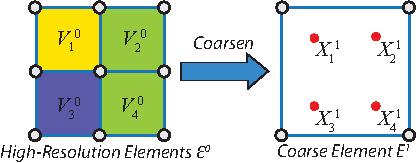
\includegraphics[width=0.6\textwidth]{images/coarseFine.pdf}
	\caption{The relationship between high-resolution and coarsened elements. At each quadrature point $\vr{X}_k^1$, the coarse element copies the corresponding energy density function $V_k^0$ from the high-resolution element.}
	\label{fig:coarseFine}
\end{figure}
We observe that even if the individual base material models are isotropic, the coarse element can become anisotropic by assigning different material parameters at the quadrature points.
We propose to improve the fitting by augmenting the coarse material model with an anisotropic term.
The complete model is then given by
\begin{align}
\begin{split}
V^1(\vr{u}^1, \, \vr{p}^1, \, C) &= \sum_{k=1}^8 \bigg( w_k \, V_k^0(\vr{u}^0, \,\vr{p}_k^1, \, \vr{X}_k^1)\\
& + C_k\left( \sqrt{\vr{v}^T\vr{F}_k^T\vr{F}_k\vr{v}} - 1\right)^2\bigg),\\
\label{eq:materialModel2}
\end{split}
\end{align}
where $\vr{v}$ is a unit-length direction of anisotropy and $C_k$ is the scaling parameter at the $k^{th}$ quadrature point. 
The gradient of the anisotropic term is
\[
\frac{d( \sqrt{\vr{v}^T\vr{F}^T\vr{F}\vr{v}} - 1)^2}{d\mathbf{F}}
=(1-\frac{1}{\|\mathbf{F}\mathbf{v}\|})\mathbf{F}\mathbf{v}\mathbf{v}^T.
\]
The second order gradient in the direction of a given $\delta \mathbf{F}$ is
\[
\left((1-\frac{1}{\|\mathbf{F}\mathbf{v}\|})\mathbf{I} 
+ \frac{1}{\|\mathbf{F}\mathbf{v}\|^3}\vr{F}\vr{v}\vr{v}^T\vr{F}^T\right)\delta\mathbf{F}^T\mathbf{v}\mathbf{v}^T.
\]
\subsection{Force Space Sampling}
\label{sec:force_space_sampling}
As mentioned previously, we take a sampling-based approach to coarse material fitting. In order to fit our model (\autoref{eq:materialModel2}) to $V^0$ we first draw a number of samples from the deformation space of $\set{E}^0$ and compute $V^0$ for each sample.
If a user has prior knowledge of the set of meshes and simulations that they will require, then the best way to draw the samples is to run a number of anticipated simulations with various material combinations.
In this paper, we provide a more general method to draw samples for a material model.
Initially, we attempted sampling by applying a random deformation to the corners of $\mathit{E}^1$; however, this led to many infeasible samples for very stiff materials.
In order to alleviate this problem we perform sampling in the force space.

For each element $\mathit{E}^0\in \, \set{E}^0$ we apply a set of randomly generated forces.
We solve an elastostatic problem to compute the deformation of $\set{E}^0$, using constraints to remove rigid motion. Recall that this is fast because $^0\set{E}$ consists of just 8 elements.
Each sample is then a tuple $\left\{\vr{u}^0, \, V^0\right\}$ (\autoref{fig:sampling}) 
where $^0\vr{u}$ are the nodal displacements of $\set{E}^0$,
and $V^0$ is the strain energy density value of this deformed configuration.
\begin{figure}
	\centering
	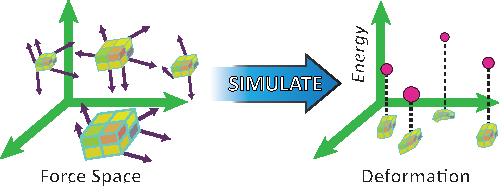
\includegraphics[width=0.6\columnwidth]{images/sampling.pdf}
	\caption{ We sample the energy function of a 2$\times$2$\times$2 block of hexahedra by applying random forces and deforming the block using FEM. Each set of forces results in a deformation-energy tuple which is used during fitting.}
	\label{fig:sampling}
\end{figure}

\subsection{Fitting}
\label{sec:fitting}
Given a set of deformation samples, $\left\{ \vr{u}^0, \,V^0\right\}$, we perform a non-negative least squares fit to determine the parameters, $\vr{p}^*$, for material model(\autoref{fig:fitting}):
\begin{align}
\vr{p}^*= \underset{\vr{p}^1}{\operatorname{argmin}} \, \sum_{s=1}^{n_s}\left(V_s^0- \, V^1\left(\vr{r}\left(\vr{u}_s^0\right), \, \vr{p}^1\right)\right)^2,
\label{eq:fitting}
\end{align}
where $\vr{r}$ constructs $\vr{u}^1$ from $\vr{u}^0$, $n_s$ is the total number of samples, and $s$ indexes all samples. In our experiments we use the simplest form of $\vr{r}$ choosing it to extract the displacements of the corners of $\set{E}^0$.
The material parameters are all constrained to be positive to improve simulation stability.
Since the material parameters have physical meanings such as Young's modulus and spring stiffness,
the non-negativity constraint specifies that the coarse material is made of traditional base materials.

\paragraph{Fitting in the Presence of Anisotropy}
If performed naively this optimization is nonlinear because we must simultaneously solve for $\vr{v}_k$, the preferred direction of anisotropy. This can severely slow the fitting procedure, especially in cases where it would otherwise be a linear least squares problem (i.e if all fine-scale materials are Neo-Hookean or a similarly simple material model).
To avoid this problem we first estimate all anisotropy directions, and then solve \autoref{eq:fitting} for the remaining material parameters.
Our intuition is that anisotropy manifests itself as preferential stretching along a particular axis. To find this axis, we apply stretching forces to a block in a discrete set of directions uniformly sampled over a sphere.
If the stretching force is close to the direction of anisotropy, then the amount of stretching deformation is reduced.
For any given stretching direction $\mathbf{v}$, we apply a stretching force and compute the deformation gradient $\mathbf{F}$ of  each quadrature point.
Under $\mathbf{F}$, a unit length vector in direction $\mathbf{v}$ is stretched to a new length $l = \|\mathbf{F}\mathbf{v}\|$.
The set of all 3D vectors $l\mathbf{v}$ forms an ellipse-like shape.
We find the principal axes of the ellipse (via SVD) and use them as directions of anisotropy.
\begin{figure}
	\centering
	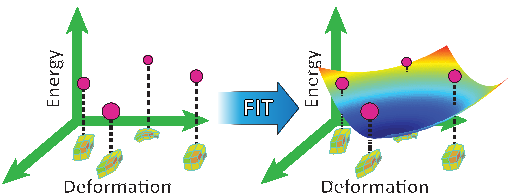
\includegraphics[width=0.6\columnwidth]{images/fitting.pdf}
	\caption{ Coarse potential energy functions are fitted to the deformation-energy samples using a least-squares optimization.}
	\label{fig:fitting}
\end{figure}
\paragraph{Regularization} Since vastly different material assignments, $^0\set{M}_k$, can produce the same coarse material, our na\"{i}ve cost function (\autoref{eq:fitting}) can produce very large parameter values and even non-physical negative ones.
For example, consider a homogeneous material assignment at the high-resolution level.
The same coarse material can be achieved by interleaving hard and soft materials at each fine element or by assigning a single, well chosen material to all fine elements.
To overcome this, we add a regularization term to control the parameter ranges and prevent overfitting of the training samples.
Our modified error function takes the following form:
\begin{equation}
\sum_{s=1}^{n_s}\left(V_s^0- \, V^1\left(\vr{r}\left(\vr{u}_s^0\right), \, \vr{p}^1\right)\right)^2 + 
\lambda\sum_k (\vr{p}_k^1 - \, \vr{p}_k^0)^2,
\end{equation}
which prevents material parameters from deviating too far from  $\set{M}_k^0$.
We chose the regularization constant $\lambda=0.02$ for the results in this paper.
In our experiments, since the base energy functions are linear with respect to the material parameters, the fitting problem can be solved by linear regression with regularization.

\begin{figure}
	\centering
	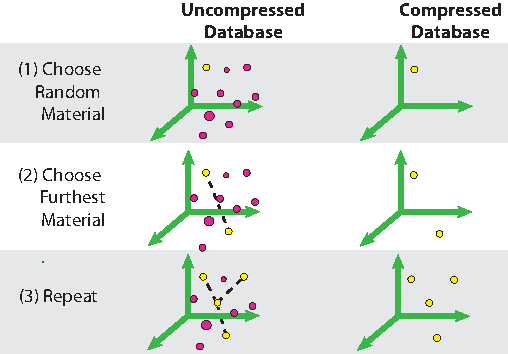
\includegraphics[width=0.6\columnwidth]{images/compression}
	\caption{Database compression step adds coarse materials to a compressed database by a farthest point sampling strategy.}
	\label{fig:compression}
\end{figure}

\subsection{Database Compression}
\label{sec:compression}
Given $n$ materials in the palette, the number of material combinations in a 2$\times$2$\times$2 block is $n^8$. In modern hardware, it is impossible to compute and store all material combinations even for a moderately-sized palette with $100$ materials.
In order to compress the number of materials stored in our coarse material database, we select a small number of representative material combinations and remove all others. We compare materials in a feature space. In order to construct coarse material feature vectors, we first select a common subset of deformations from all computed deformation samples. We then evaluate the potential energies of each coarse material at each deformation sample. The stacked vector of energies becomes a coarse material feature vector. 

Since our base materials differ in stiffness by orders of magnitude, we take the logarithm to measure the difference in ratio.
Let $D$ be the $L^2$ norm of log-energies between the two materials given by
\begin{equation}
D(A,B)=\sqrt{\sum_s (\log(V^{A}_{s})-\log(V^{B}_{s}))^2},
\end{equation} where $A$ and $B$ denote two distinct coarse materials in the database. 
Given the distance metric, we can select $k$ representatives materials using farthest point sampling~\cite{eldar1997farthest}. We randomly choose an initial coarse material and then repeatedly select the material combination furthest away from any previous representatives -- continuing until we obtain $k$ representatives (\autoref{fig:compression}). This compression algorithm chooses $k$ samples that equally cover the coarse material energy space, helping to preserve good behavior in our coarse simulations. 
\subsection{Hierarchical Coarsening}
While one level of coarsening can yield significant speed-ups, DDFEM can also be applied hierarchically.
As discussed in~\autoref{sec:compression}, the exponential growth of coarse material palettes at each level makes it prohibitively expensive to perform fitting.
We address this by changing our coarsening strategy. 
Instead of choosing $\set{E}^0$ to be a 2$\times$2$\times$2 block we choose it to be a 2$\times$1$\times$1 block, which we coarsen. We construct an intermediate database of materials and compress. 
We then choose $\set{E}^0$ to be a 1$\times$2$\times$1 block, coarsen and compress, and finally a 1$\times$1$\times$2 block, coarsen and compress. Intermediate compression greatly reduces the number of samples we need to generate in order to populate the material parameter database for the next coarsening level. 
It is important to note that our intermediate databases only store lookup tables which allow us to extract appropriate material IDs for the next coarsening stage. Material parameters need only be stored in the final database since it is these elements that are simulated.
\begin{figure}
	\centering
	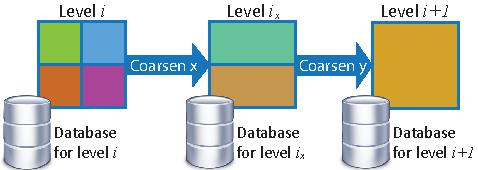
\includegraphics[width=0.7\textwidth]{images/hierchical}
	\caption{Hierarchical coarsening operates on one dimension at a time, performing clustering at each intermediate stage (here denoted $i_x$). This allows our compression algorithm to be applied aggressively, greatly reducing the number of energy samples we need for fitting material parameters. }
	\label{fig:hierarchy}
\end{figure}
\section{Runtime Simulation}
\label{sec:runtime}
Once our coarse material database, $\set{P}^1$, has been constructed we can use it to perform fast online coarsening. 
Initially, the user loads geometry which is embedded in a hexahedral grid for simulation. Prior to simulation we iterate over all 2$\times$2$\times$2 blocks of hexahedral elements and perform mesh coarsening by replacing these 8 elements with a single coarse element. We perform a database lookup into $\set{P}^1$, using the material ID numbers of the 8 original elements, to quickly retrieve the optimal coarse material for this coarse element. Database lookup is fast (even using our unoptimized, single-threaded implementation), and this is what makes DDFEM so appealing.
We achieve significant simulation speed-up from coarsening, retain accuracy in the simulation, and reduce the cost of material coarsening at runtime to a negligible amount.
	Our material model can be used in any simulation algorithm suitable for non-linear elasticity. In our experiments, we use Coin-IpOpt~\cite{ipopt} to implement static and dynamics simulations with tolerance (``tol'' option) set to $0.5$. We use Pardiso as our linear solver.
	For timing purposes, we limit Pardiso to single thread mode.
	The pseudo-code for static simulation is shown in~\autoref{alg:sim}.
\begin{algorithm}
	\caption{Static Simulation}\label{alg:sim}
	\begin{algorithmic}[1]
		\REPEAT
		\STATE $\mathbf{f}$: global force vector
		\STATE $L$: triplet list for global stiffness matrix
		\FOR{each element e}
		\STATE compute elastic force $\mathbf{f}_e$
		\STATE add $\mathbf{f}_e$ to $\mathbf{f}$
		\ENDFOR
		\STATE add external force $\mathbf{f}_{ext}$ to $\mathbf{f}$
		\FOR{each element e}
		\STATE $\mathbf{K}_e$: element stiffness matrix
		\FOR{each quadrature point q}
		\STATE compute stiffness matrix $\mathbf{K}_q$ at quadrature point
		\STATE $\mathbf{K}_e+=\mathbf{K}_q$
		\ENDFOR
		\STATE append entries of $\mathbf{K}_e$ to $L$
		\ENDFOR
		\STATE sort $L$ to get sparse stiffness matrix $\mathbf{K}$
		\STATE set entries in $\mathbf{K}$ and $\mathbf{f}$ for fixed vertices
		\STATE $\Delta\mathbf{x}=\mathbf{K}^{-1}\mathbf{f}$
		\STATE compute step size $h$ using line-search
		\STATE $\mathbf{x}+=h\Delta\mathbf{x}$
		\UNTIL{convergence}
	\end{algorithmic}
\end{algorithm}

\begin{table}[!h]
	\centering
	\footnotesize
	\begin{tabular}{l c r r r r r r r r}
		\hline 
		\textbf{Example} &\textbf{grid size}&\textbf{rel sp}&\textbf{time/iter}&\textbf{iters}&\textbf{error}\\
		\hline
		{\color{HiResColor}Pushing(0)} &16$\times$16$\times$16&1.0 &1.010 &5&-\\
		{\color{DDFEMColor}Pushing(1)} &8$\times$8$\times$8   &11.5&0.087&5&8.91e-4\\
		{\color{DDFEMColor}Pushing(2)} &4$\times$4$\times$4   &31.4&0.032&5&1.36e-2\\
		\hline 
		{\color{HiResColor}Bending(0)} &8$\times$32$\times$8&1.0   &0.270 &28&-\\
		{\color{DDFEMColor}Bending(1)} &4$\times$16$\times$4&12.6  &0.028 & 22& 5.60e-2\\
		{\color{DDFEMColor}Bending(2)} &2$\times$8$\times$2 &22.7  &0.015 & 22&8.88e-2\\
		\hline 
		{\color{HiResColor}Twisting(0)} &8$\times$32$\times$8&1.0  & 0.300 & 16&-\\
		{\color{DDFEMColor}Twisting(1)} &4$\times$16$\times$4&15.2 & 0.031 & 10&1.56e-2\\
		{\color{DDFEMColor}Twisting(2)} &2$\times$8$\times$2 &20.7 & 0.019 & 12&3.28e-2\\
		\hline
		{\color{HiResColor}Buckling(0)} &128$\times$8$\times$16&1.0   &8.85 &32&-\\
		{\color{DDFEMColor}Buckling(1)} &64$\times$4$\times$8  &50.1 &0.28 &20&7.24e-3\\
		{\color{DDFEMColor}Buckling(2) }&32$\times$2$\times$4  &331.8&0.12 &7 &3.14e-2\\
		\hline
		{\color{HiResColor}Fibers(0)} &32$\times$100$\times$32&1.0  &193.85&17&-\\
		{\color{DDFEMColor}Fibers(1)} &16$\times$50$\times$16 &51.2 &4.95  &13& 2.94e-2\\
		{\color{DDFEMColor}Fibers(2)} &8$\times$25$\times$8   &489.5&0.96  &7 & 4.26e-2\\
		\hline
		{\color{HiResColor}Bridge(0)} &56177&1.0&43.44&14&-\\
		{\color{DDFEMColor}Bridge(1)} &9727&8.4&4.88&15&4.39e-3\\
		{\color{HiResColor}Bridge-arch(0)} &65684&1.0&54.99&3&-\\
		{\color{DDFEMColor}Bridge-arch(1)} &11695&8.1&7.84&3&3.68e-4\\
		\hline
		{\color{HiResColor}George(0)} &46152 & 1.0&52.19&23&-\\
		{\color{DDFEMColor}George(1)} &6755 & 16.4&3.49&21&2.86e-2\\
		{\color{HiResColor}George-bone(0)} &46152 & 1.0&41.35&12&-\\
		{\color{DDFEMColor}George-bone(1)} &6755 & 13.2&2.70&14&2.99e-2\\
		\hline
	\end{tabular}
	\vspace{-4pt}
	\caption{Relative performance, absolute performance in seconds and average vertex error relative to the bounding box size for full-resolution and coarsened simulations.
		Relative performance illustrates the performance increase gained by coarsening with respect to the time taken for the high-resolution static simulation to converge. Bracketed numbers after each example name indicate the number of coarsening levels with 0 indicating the {\color{HiResColor}high-resolution} simulation. All computation times are recorded using Coin-IpOpt running in single threaded mode on a 2.5 GHz Intel Core i7 processor. }
	\label{table:performance}
\end{table}
\begin{figure}[t]
	\centering
	\begin{tabularx}{0.92\columnwidth}{ Y Y }
		\textbf{Pushing} & \textbf{Twisting} \\
		\textbf{12x Faster} & \textbf{15x Faster}
	\end{tabularx}\\
	\subcaptionbox{}{
		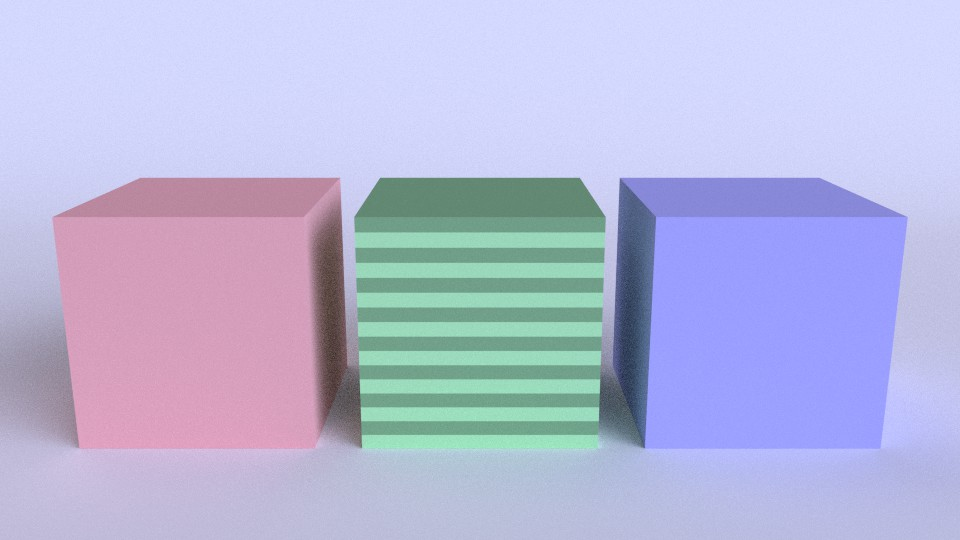
\includegraphics[width=0.45\textwidth]{images/push_l1_begin}
	}%\vrule
	\subcaptionbox{}{
		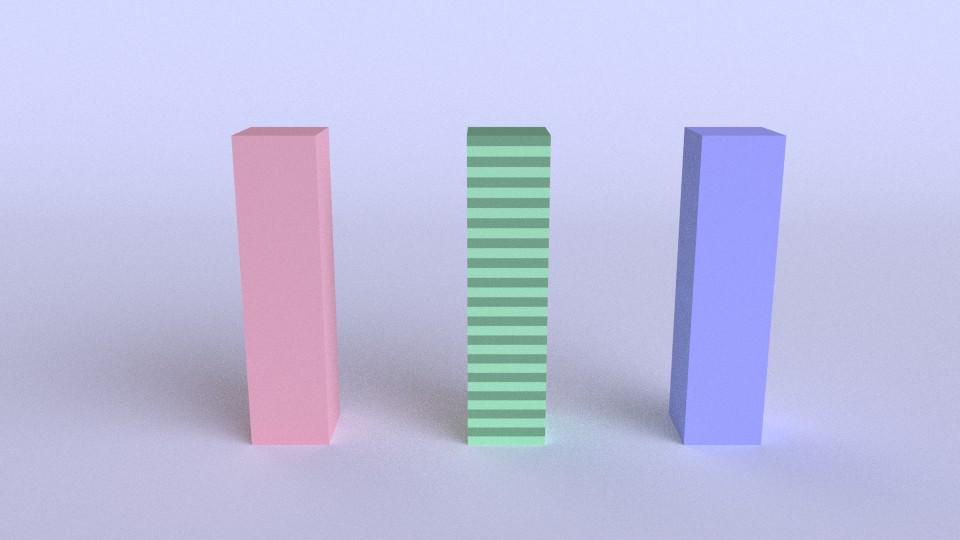
\includegraphics[width=0.45\textwidth]{images/twist_l1_begin}
	}
	\\
	\subcaptionbox{}{
		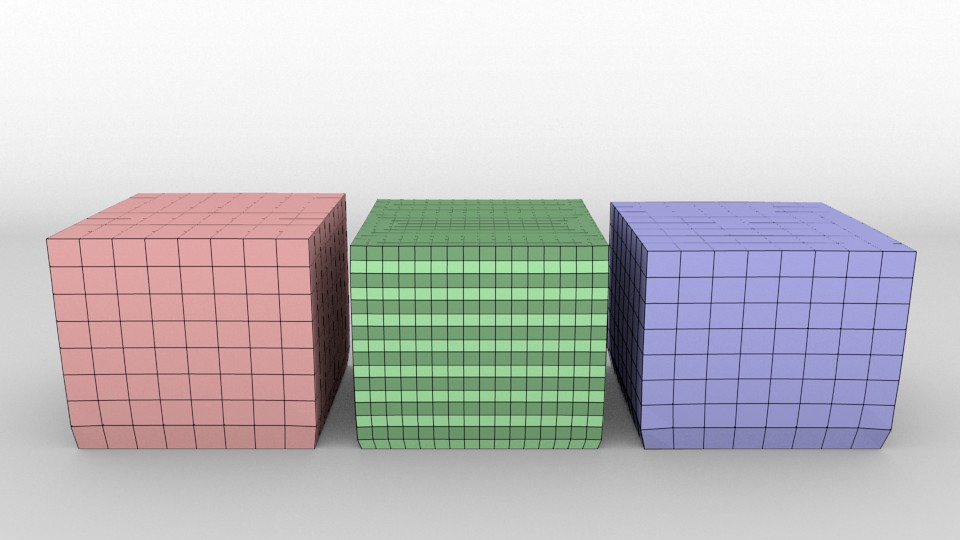
\includegraphics[width=0.45\textwidth]{images/push_l1_wire_end}
	}%\vrule
	\subcaptionbox{}{
		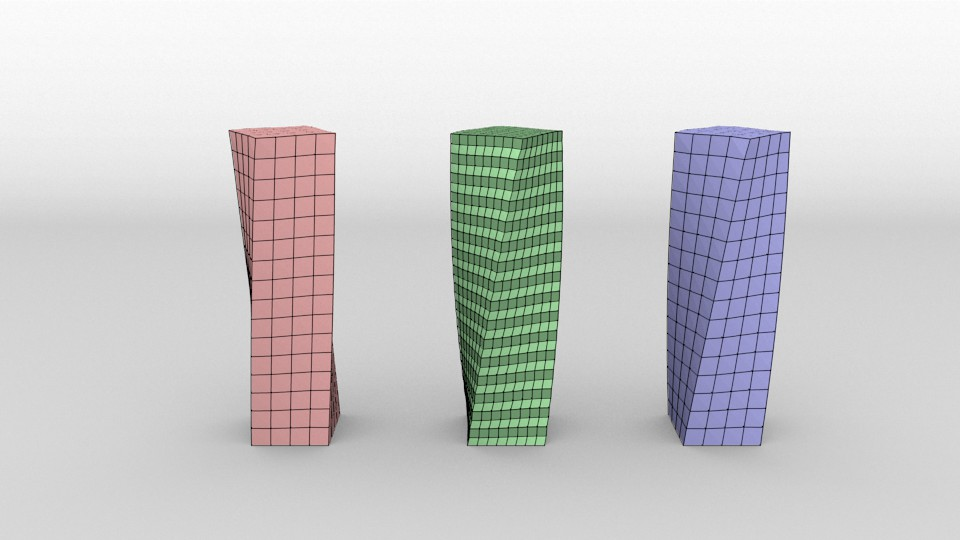
\includegraphics[width=0.45\textwidth]{images/twist_l1_wire_end}
	}
	%\vspace{-3mm}
	\caption{Examples of pushing a cube (a - Initial State, c - Compressed) and twisting a bar (b - Initial State, d - Compressed), both with heterogeneous material distribution. We compare {\DDFEM} to {\Naive} and the  ground-truth, {\HiRes}. We render wire frames to show the simulation meshes.}
	\label{fig:accuracy}
\end{figure}
\begin{figure}[t]
	\centering
	\begin{tabularx}{0.92\columnwidth}{ Y Y }
		\textbf{1 Level of Coarsening} & \textbf{\textbf{2 Levels of Coarsening}} \\
		\textbf{13x Faster} & \textbf{23x Faster}
	\end{tabularx}\\
	\subcaptionbox{}{
		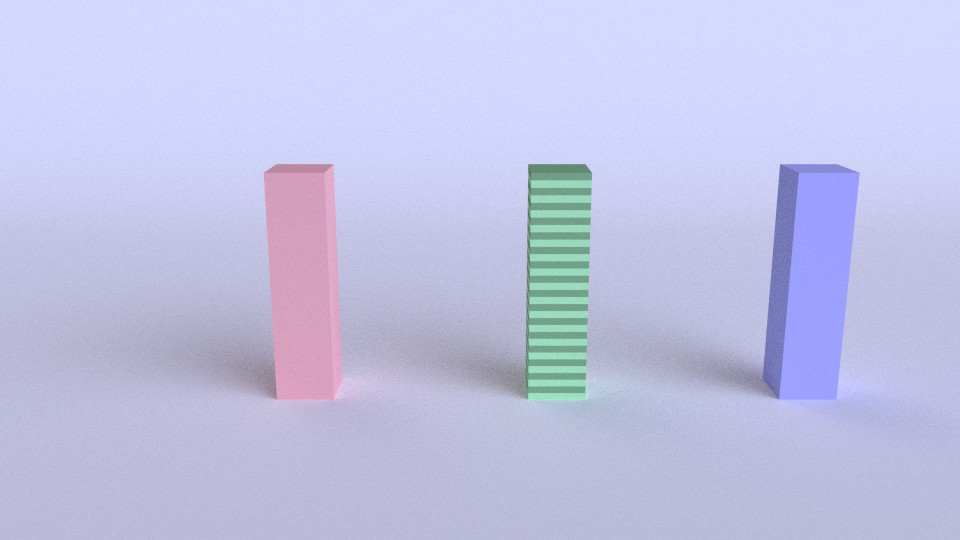
\includegraphics[width=0.47\columnwidth, trim=170px 105px 40px 105px, clip=true]{images/bend_l1_begin}
	}
	%\vrule
	\subcaptionbox{}{
		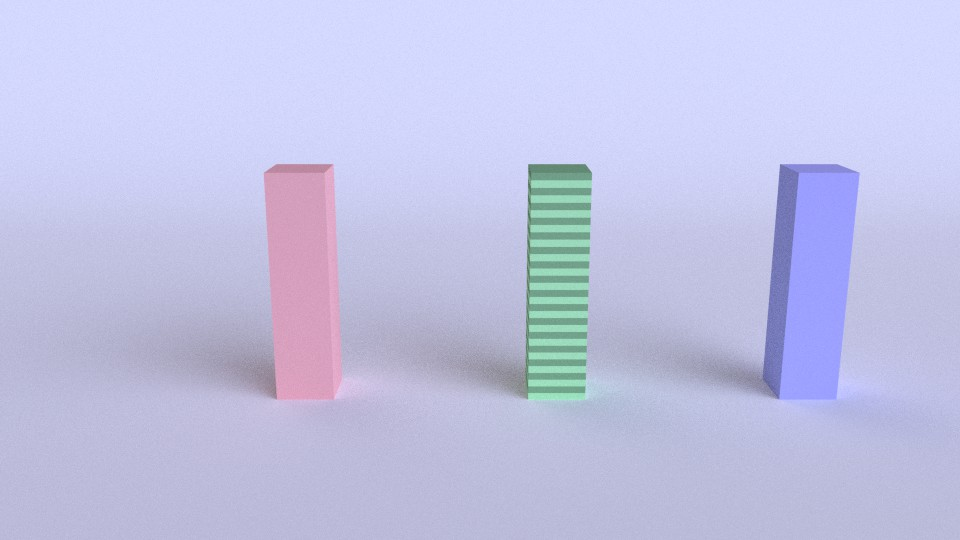
\includegraphics[width=0.47\columnwidth, trim=170px 105px 40px 105px, clip=true]{images/bend_l2_begin}
	}\\
	\subcaptionbox{}{
		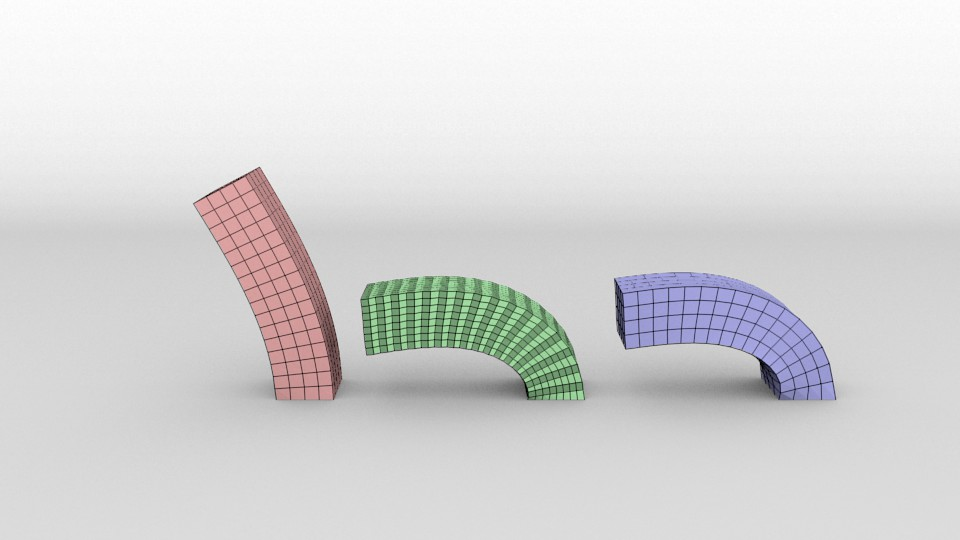
\includegraphics[width=0.47\columnwidth, trim=170px 105px 40px 105px, clip=true]{images/bend_l1_wire_end}
	}
	%\vrule
	\subcaptionbox{}{
		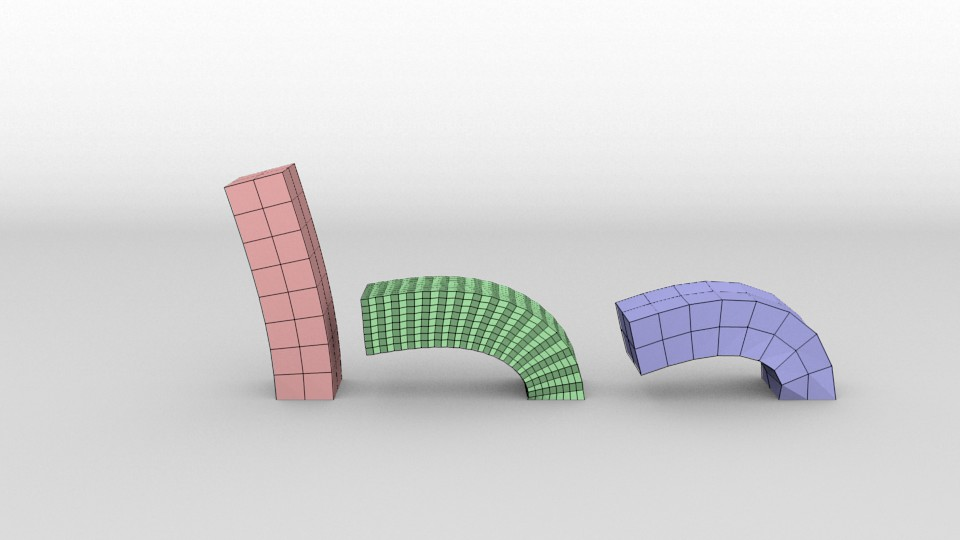
\includegraphics[width=0.47\columnwidth, trim=170px 105px 40px 105px, clip=true]{images/bend_l2_wire_end}
	}
	%\vspace{-8pt}
	\caption{Bending a heterogeneous bar: We compare {\DDFEM} to {\Naive} and a {\HiRes}. Subfigures (a, c) show comparison for 
		1 level of coarsening, and (b, d) show 2 levels of
		coarsening. The na\"{i}ve coarsening
		approach results in a much stiffer behavior, whereas our fitted
		model more closely approximates the fine model.}
	\label{fig:bending}
\end{figure}
\begin{figure}[t]
	\centering
	\begin{tabularx}{0.92\columnwidth}{ Y Y }
		\textbf{1 Level of Coarsening} & \textbf{\textbf{2 Levels of Coarsening}} \\
		\textbf{50x Faster} & \textbf{332x Faster}
	\end{tabularx}\\
	\subcaptionbox{}{
		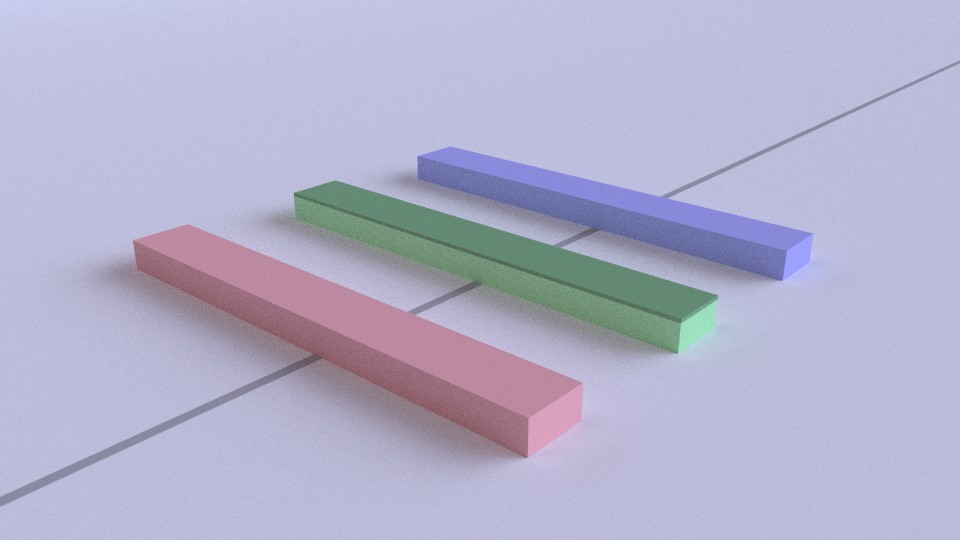
\includegraphics[width=0.47\columnwidth, trim=105px 60px 70px 115px, clip=true]{images/buckle_l1_begin}
	}%\vrule
	\subcaptionbox{}{
		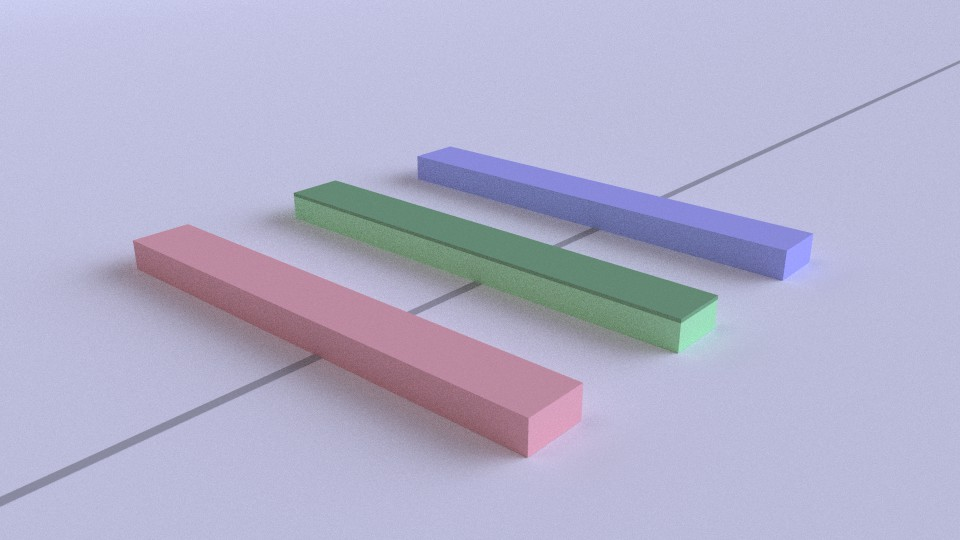
\includegraphics[width=0.47\columnwidth, trim=105px 60px 70px 115px, clip=true]{images/buckle_l2_begin}
	}
	\\
	\subcaptionbox{}{
		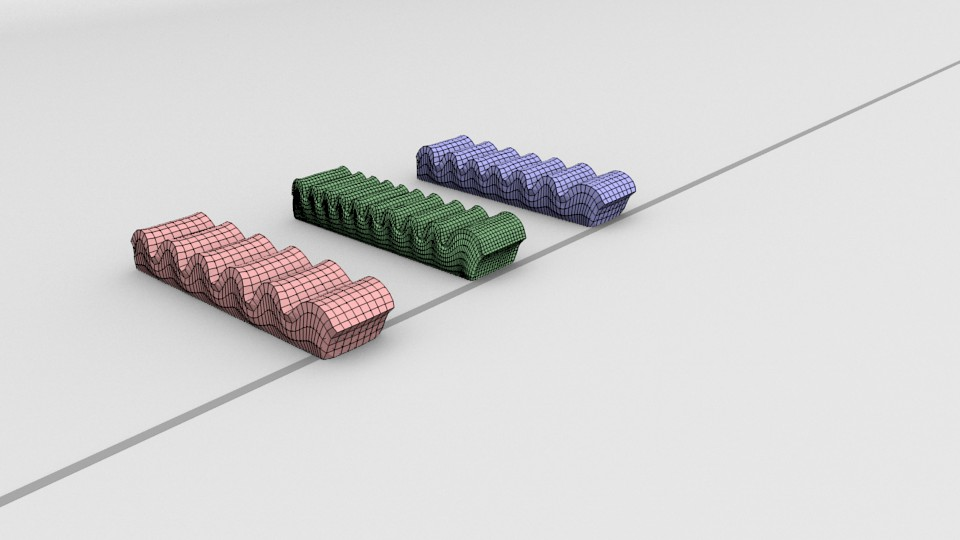
\includegraphics[width=0.47\columnwidth, trim=105px 60px 70px 115px, clip=true]{images/buckle_l1_wire_end}
	}
	%\vrule
	\subcaptionbox{}{
		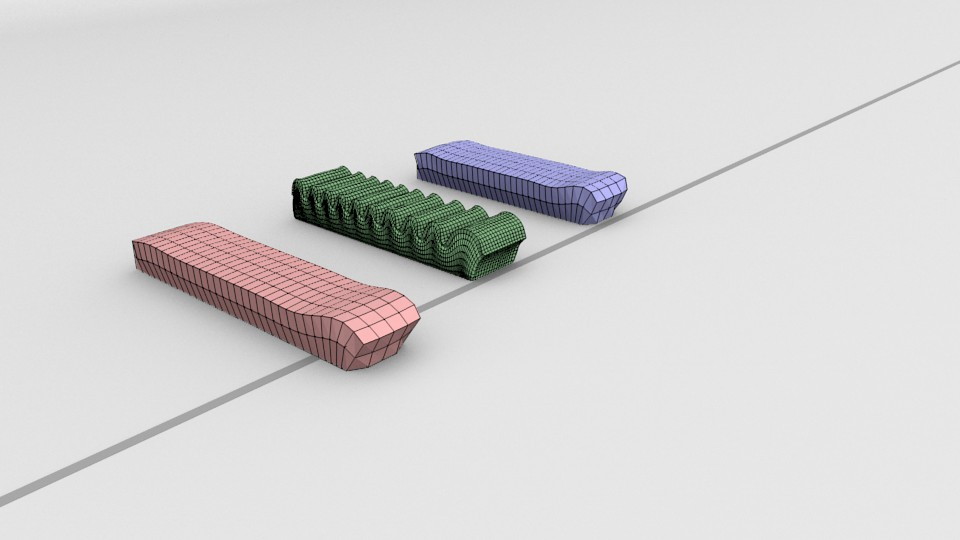
\includegraphics[width=0.47\columnwidth, trim=105px 60px 70px 115px, clip=true]{images/buckle_l2_wire_end}
	}
	\vspace{-2pt}
	\caption{Compressing a heterogeneous slab using {\Naive} (1 level and 2 levels of coarsening), {\DDFEM} (1 level and 2 levels of coarsening) and a {\HiRes}. The top, darker layer is stiffer, causing the object to buckle. The bottom vertices are constrained to stay on the floor. Figure (a,b) shows the slabs before compression, figure (c,d) shows the slabs after compression and figure. Notice that, after 1 level of coarsening, {\Naive} neither compresses nor buckles as much as either {\DDFEM} or {\HiRes}. After 2 levels of coarsening, \note{the buckling behavior is lost.}
		The {\Naive} fails to capture the compressive behavior of {\HiRes}, whereas {\DDFEM} does.}
	\label{fig:buckling}
\end{figure}
\begin{figure}
	\centering
	\begin{tabularx}{0.92\columnwidth}{ Y Y }
		\textbf{1 Level of Coarsening} & \textbf{\textbf{2 Levels of Coarsening}} \\
		\textbf{51x Faster} & \textbf{489x Faster}
	\end{tabularx}\\
	\subcaptionbox{}{
		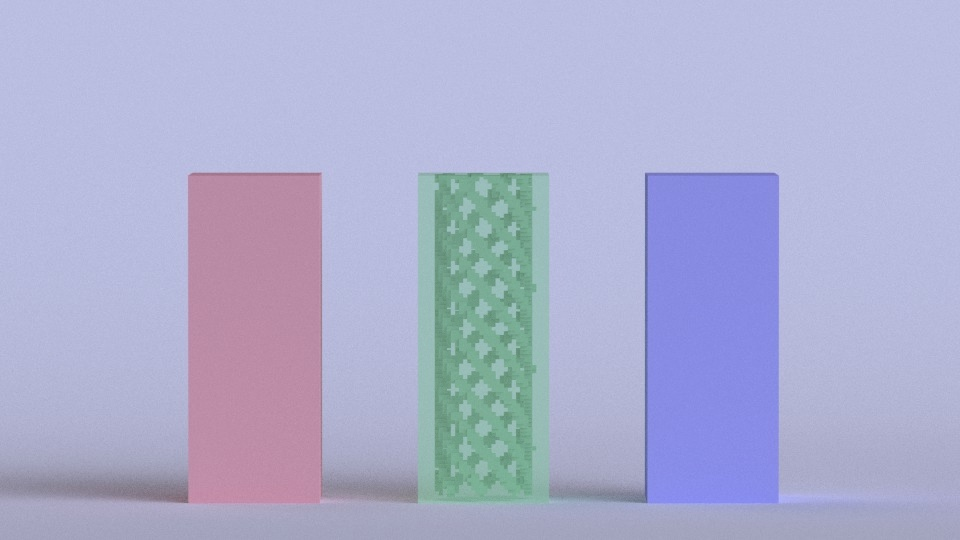
\includegraphics[width=0.4\textwidth]{images/fiber_l1_xray_begin}
	}%\vrule
	\subcaptionbox{}{
		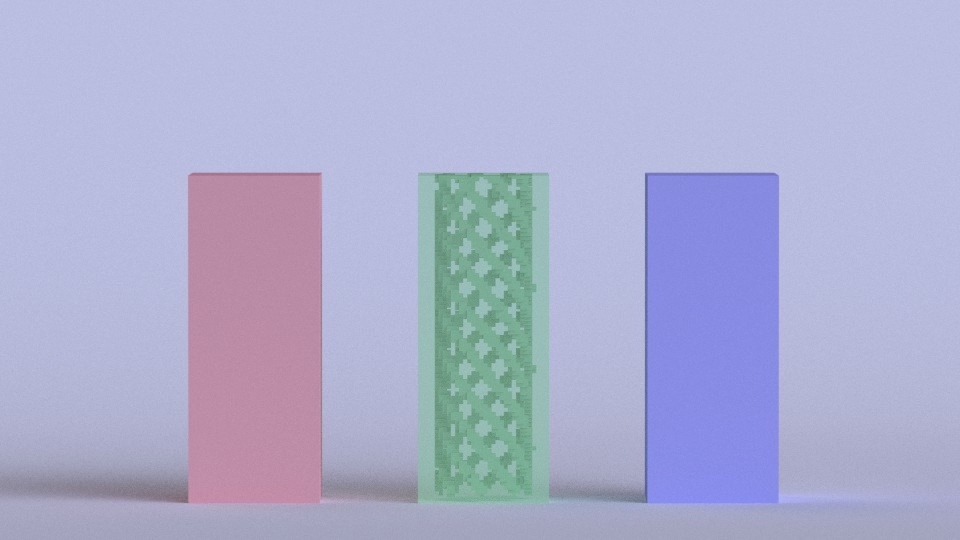
\includegraphics[width=0.4\textwidth]{images/fiber_l2_xray_begin}
	}  \\

	\subcaptionbox{}{
		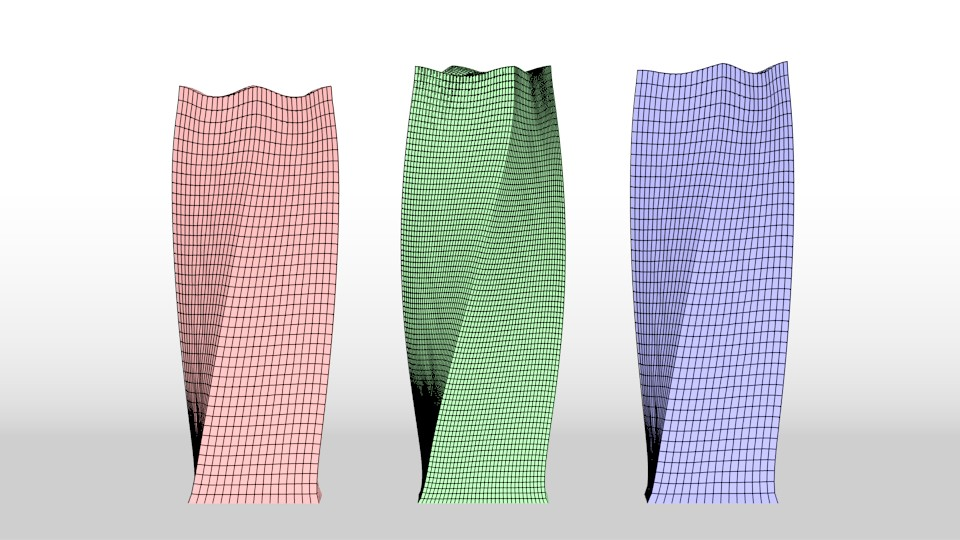
\includegraphics[width=0.4\textwidth]{images/fiber_l1_wire_end}
	}%\vrule
	\subcaptionbox{}{
		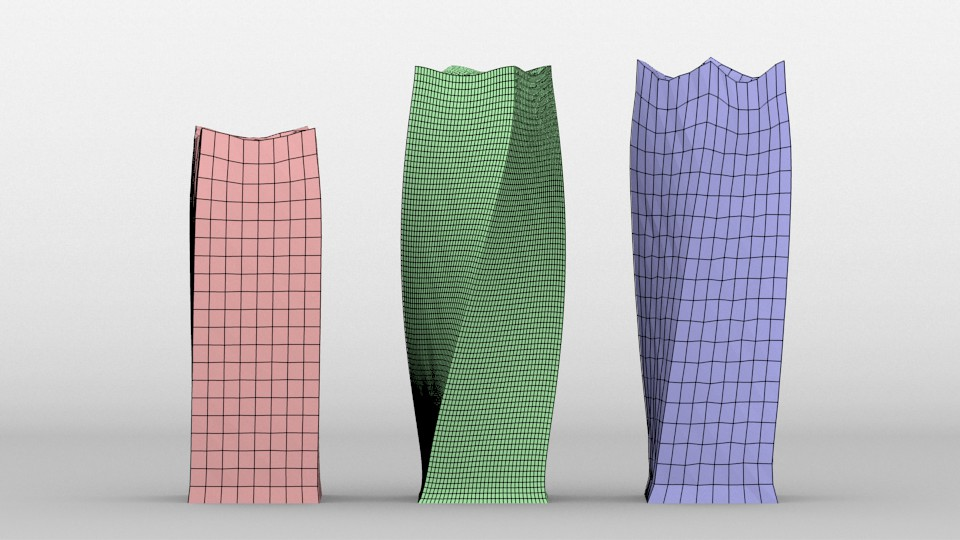
\includegraphics[width=0.4\textwidth]{images/fiber_l2_wire_end}
	}
	\vspace{-2pt}
	\caption{Simulating a bar with an embedded set of fibers using {\Naive}, {\DDFEM} and a {\HiRes}. Note that {\DDFEM} captures the characteristic twisting motion of the bar better than {\Naive}.  (a,b) shows the initial state of both bars while (c,d) shows the deformed state after pulling on the top of the bars.}
	\label{fig:fiberPull}
\end{figure}
\section{Results and Discussion}
\label{sec:result}
All the results shown here are simulated using nonlinear constitutive models at the fine scale. This and coarsening speed are the key differentiating factors between DDFEM and other coarsening algorithms such as~\citet{Nesme2009} and~\citet{Kharevych2009}.
\note{Our database starts with three Neo-hookean base materials with Young's modulus $1e5, 1e6, 1e7$ and Poisson's ration $0.45$. For comparison with 3D-printed objects, we used two base materials with measured Young's moduli.
	We use $500$ force directions, and sample $5$ magnitudes in each direction,
	resulting in $2500$ force samples for each material combination.
	In addition, we generate $500$ stretching samples for computing the direction of anisotropy. During fitting, we use shear modulus and Lam\'{e}'s first parameter,
	as well as the spring stiffness.
	We repeat the same process for the second level of coarsening, using
	$6561$ materials in the first level as base materials. We select
	$400$ representatives at each intermediate level.}

\subsection{Database}
One advantage of our compact coarse material representation is the small amount of storage it requires. In fact we require only $6\times8=48$ floating-point values for each material at the first coarsening level and $6\times64=384$ values for the second level.
(For each finer element, $^0\vr{p}$ contains 2 material moduli plus $C, \vr{v}$.)
For further recursive levels, we can limit ourselves to $320$ values per material.
Our current 3 material database is $4$ megabytes in size.

\subsection{Simulation Results}
We show results from elastostatic simulations performed using DDFEM. We also demonstrate its performance advantages over high-resolution simulations. We render wire frames to show the discretizations of the high-resolution and coarse meshes. We first show examples of two simple simulations, the pushing and twisting of a rectangular object with heterogeneous, layered material distribution (\autoref{fig:accuracy}). Note that in all cases DDFEM qualitatively matches the behavior of the high-resolution simulation. We also compare the performance of DDFEM to a na\"{i}ve coarsening method that uses the material properties from 2$\times$2$\times$2 element blocks of the high-resolution simulation mesh at each corresponding quadrature point. \note{In our supplemental video we compare to a second baseline model which averages material parameters inside each coarse element. This average model is less accurate than the Na\"{i}ve model in all cases.} 

Na\"{i}ve approaches often exhibit pathological stiffness  for heterogeneous materials (illustrated by the lack of compression of the box and lack of twisting of the bar)~\cite{Nesme2009}. In these cases, DDFEM yields good speed ups while maintaining accuracy. For a single level of coarsening we achieve \emph{8 times or greater} speed ups for all examples. Performance numbers and mean errors are listed in \autoref{table:performance}.
Since the fine simulation and the coarse simulation have different numbers of vertices, we create a fine mesh from the coarse simulation by
trilinearly interpolating the fine vertices using the coarse displacements. The errors are measured by computing the average vertex distance relative
to the longest dimension of the bounding box in rest shape.
We also examine the behavior of DDFEM during bending (\autoref{fig:bending}). Yet again the na\"{i}ve coarsening method completely fails to capture the behavior of the high-resolution result, while DDFEM offers a much better approximation. 
\paragraph{Performance Analysis}
\note{\autoref{table:quadPerformance} shows time spent in quadrature evaluation versus in solver at coarse and fine levels.
	We use $8$ quadrature points for the first level of coarsening 
	and $64$ for the second level. The time for computing the local stiffness matrix for one element increases from $0.1$ms to $1$ms.
	In the second level, the speedup comes from the reduced number of elements over which to perform quadrature and the time required for the linear solver.
	
	To further investigate the performance of our coarsened simulations
	we replaced Pardiso with an assembly-free
	Jacobi-preconditioned conjugate gradient (CG) linear solver and used this to simulate our George-bone test case.
	While the overall runtime of the high-resolution simulation increased from $496$ to $2082$ seconds (most likely do to the unoptimized nature of our solver) our coarsened model achieved 20x and 67x speedups using one level and two levels of coarsening respectively. 
	One might expect no benefit from the second level of coarsening since the 
	number of quadrature points remains constant. 
	However, the number of CG iterations is roughly proportional to the number of vertices in the simulation mesh and thus the coarse model converges more quickly~(\autoref{fig:cg}).
	Since our coarse material models are not restricted to use
	a fixed number of quadrature points,
	one could design coarse models that are more tailored towards
	assembly-free solvers by reducing the number of quadrature points and simplifying the strain energy expressions.
}

\begin{figure}
	\centering
	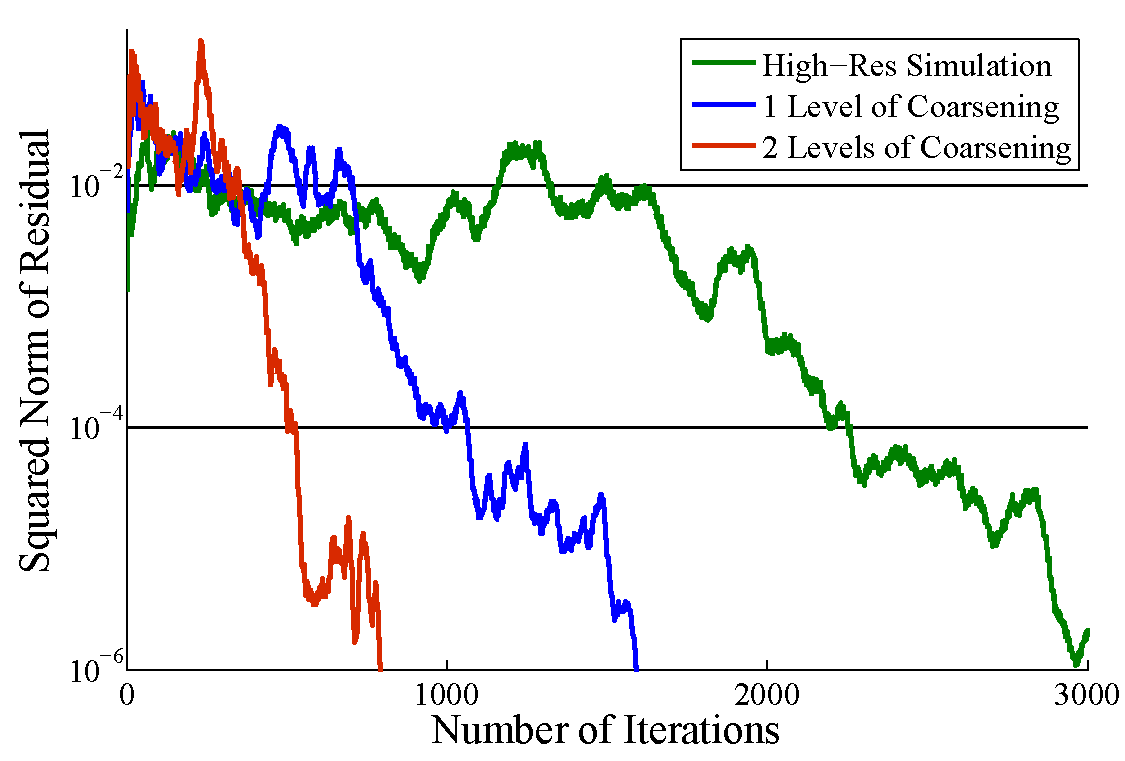
\includegraphics[width=0.6\textwidth]{figs/CGConverge.pdf}
	\caption{
		\note{Comparison of CG iterations on high-resolution and coarsened meshes of the George-bone example.
			The squared residual is measured as $\|\mathbf{K}\mathbf{x}-\mathbf{f}\|^2$.
			We observe that CG converges much faster on coarse meshes.
		}
	}\label{fig:cg}
\end{figure}

\begin{table}
	\centering
	\footnotesize
	\begin{tabular}{l c p{1cm} p{1cm} r }
		\hline 
		\textbf{Example} &\textbf{grid size}&\textbf{quad/iter} (12)&\textbf{time/iter} (2-21)&\textbf{iters}\\
		\hline 
		{\color{HiResColor}Bending(0)} &8$\times$32$\times$8   &  0.11  &0.27 &28\\
		{\color{DDFEMColor}Bending(1)} &4$\times$16$\times$4   &  0.015 &0.028&22\\
		{\color{DDFEMColor}Bending(2)} &2$\times$8$\times$2    &  0.014 &0.015&22\\
		\hline
		{\color{HiResColor}Buckling(0)} &128$\times$8$\times$16&  1.0   &8.8 &32\\
		{\color{DDFEMColor}Buckling(1)} &64$\times$4$\times$8  &  0.11  &0.28&20\\
		{\color{DDFEMColor}Buckling(2) }&32$\times$2$\times$4  &  0.10  &0.12&7\\
		\hline
		{\color{HiResColor}Fibers(0)} &32$\times$100$\times$32 & 10.0   &193&17\\
		{\color{DDFEMColor}Fibers(1)} &16$\times$50$\times$16  &  1.0   &4.9&13\\
		{\color{DDFEMColor}Fibers(2)} &8$\times$25$\times$8    &  0.68  &0.96&7\\
		\hline
	\end{tabular}
	\caption{\note{Portion of time in seconds used by quadrature computation during static simulation in seconds. Bracketed numbers indicate corresponding lines in Algorithm \ref{alg:sim}.}}
	\label{table:quadPerformance}
\end{table}
\paragraph{Complex material behavior} DDFEM can capture the gross behavior of  complex, spatially-varying material distributions. \autoref{fig:buckling} shows the results of applying DDFEM to a non-linearly elastic slab with a stiff ``skin.'' The bottom of the slab is constrained to slide along the ground with one end fixed. When force is applied to the free end of the slab, buckling occurs.  Somewhat obviously, DDFEM cannot replicate the frequency of the high-resolution buckling pattern due to the coarseness of the simulation mesh. However, it correctly captures the gross behavior of the bar and approximates the overall amount of compression well. \autoref{fig:buckling} also shows a comparison with 2nd level coarsening. In this case, the overall compression of the bar is still captured accurately. For this example DDFEM affords \emph{50 times} (1 level of coarsening) and \emph{332 times}  (2 levels of coarsening) performance improvements over the high-resolution simulation.  The artificial stiffness of the na\"{i}ve model can be seen in the reduced buckling and compression when compared to DDFEM at both coarsening levels.
%\vspace{-8pt}
\paragraph{Anisotropic material distribution} Next we explore the ability of DDFEM to handle highly anisotropic material distributions (\autoref{fig:fiberPull}). Specifically, we embed a helical set of stiff fibers in a soft, non-linearly elastic matrix. Pulling on the object induces a twisting. Again, at one coarsening level DDFEM captures this anisotropic behavior well, much better than the naive approach, and gains a \emph{51 times} speed up over the high-resolution simulation. Worth noting is that the DDFEM bar is slightly softer in the $y$-direction. This kind of inaccuracy should be expected. Since our method builds a low-dimensional approximation of a potential energy function we cannot hope to accurately reproduce the complete behavior of the high-resolution simulation.  What is important is that DDFEM captures the salient global behavior, in this case, the twisting of the bar. 
\paragraph{Geometry and material design} We present three examples of using DDFEM for geometry and material design. In the first example, we edit the material composition of the sole of a running shoe in order to stabilize it. \autoref{fig:shoe} shows the effect of the three material edits as well as relative speed up achieved over the full resolution simulation and coarsening time. DDFEM performance is always an order of magnitude more than that of the high-resolution simulation, and, most importantly, our coarsening times are on the order of milliseconds. We stress that our current implementation is completely single threaded and that coarsening, which in our case involves a simple database lookup, is inherently parallel.
In the second example, we add a supporting arch to a bridge. Prior to the addition of the support structure, the bridge sags catastrophically. The fast coarsening of DDFEM allows us to achieve an 8 fold increase in simulation performance using a single coarsening pass. In the third example, we add a rigid skeleton to a deformable character (George) in order  to control his pose. Here our single threaded, data-driven coarsening only takes ~200ms.  
\begin{figure}
	\centering
	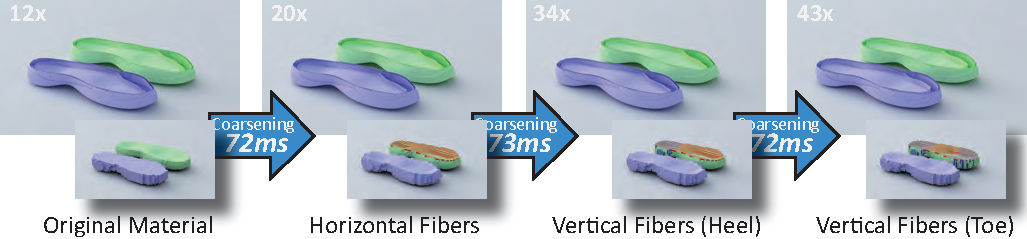
\includegraphics[width=0.90\textwidth]{images/DesignExampleShoe}
	\caption{Designing a shoe sole: We compare the performance of {\DDFEM} to that of {\HiRes} in the context of a material design problems. Large images show the effect of material changes on the sole of the shoe, which is being deformed under a ``foot-like'' pressure field. Inset images show the materials assigned to the shoe sole and the embedded finite element simulation mesh. Numbers within arrows show coarsening times between editing steps and the numbers in the upper left corner of each image show the relative performance of {\DDFEM} to  {\HiRes}. While the {\DDFEM} sole is made up of many coarse material, we display it as a single color to distinguish it from the {\HiRes}.}
	\label{fig:shoe}
\end{figure}

\begin{figure}
	\centering
	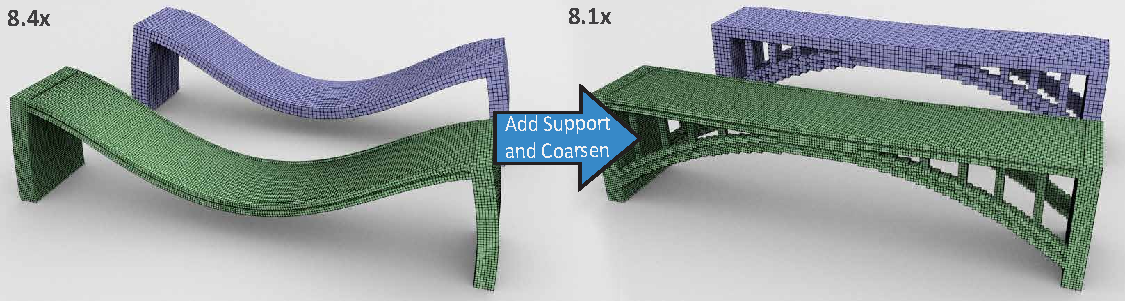
\includegraphics[width=0.8\textwidth]{images/bridge.pdf}
	\caption{Accelerating geometry change: We repair a structurally unsound bridge by adding a supporting arch (8x faster).}
	\label{fig:bridge}
\end{figure}
\begin{figure}
	\centering
	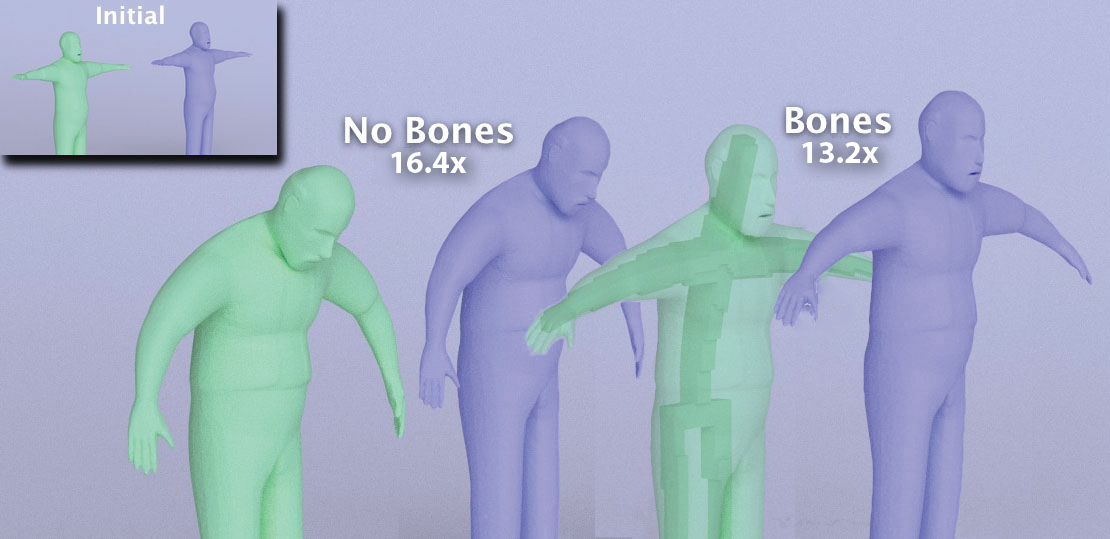
\includegraphics[width=0.8\textwidth]{images/georgeUpdate.png}
	\caption{Correcting George's posture using a rigid skeleton ({\HiRes} and {\DDFEM}).}
	\label{fig:george}
\end{figure}
\paragraph{Dynamics} Though the examples shown in this paper focus on static analysis, DDFEM is equally applicable to dynamic simulations. At its core, DDFEM simply supplies new, more accurate material models for use during simulation. This makes the method useful for accelerating various animation tasks as well. In the accompanying videos we show a dynamic simulation of our fiber embedded bar, computed using a standard linearly-implicit time integrator.

\begin{figure}
	\centering
	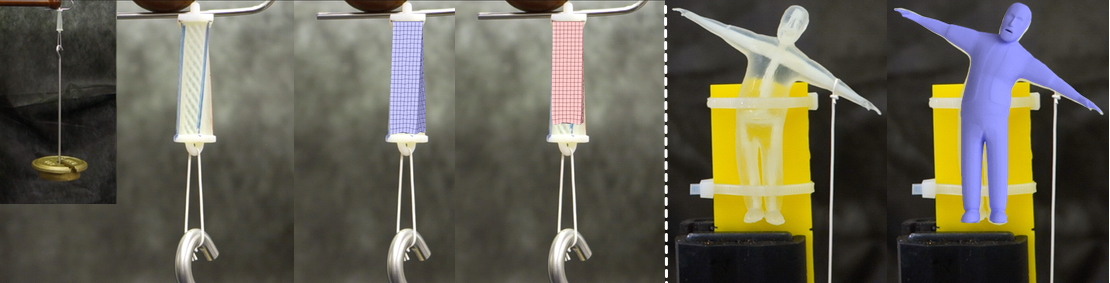
\includegraphics[width=0.8\textwidth]{images/experiments.jpg}
	\caption{A comparison of  {\DDFEM} (2 levels of coarsening) to real world deformations of 3D printed, multi-material designs. {\DDFEM} captures the twisting behavior of an anisotropic bar much more accurately than {\Naive}. Similarly {\DDFEM} accurately predicts the deformation of our heterogeneous George character. }
	\label{fig:experiments}
\end{figure}

\subsection{Fabricated Results}
Finally, we test the accuracy of our simulation against fabricated results, created using a Stratysys Object Connex 500 multimaterial 3D printer. We fabricated a bar with embedded helical fibers as well as our George character and applied specified loads to both. We show qualitative comparison of the deformed configurations of these real-world examples to our simulated results (\emph{2 levels of coarsening}-\autoref{fig:experiments}). Note that the simulation does an excellent job of predicting the deformed configuration of both objects.

\section{Limitations and Future Work}
Because DDFEM relies on a database compression step to combat the combinatorial explosion of coarse materials,  accuracy is heavily influenced by the set of representative coarse materials. Finding a better way to select coarse structures is an interesting area of future work.
Second, in our attempt to make our method geometry independent, some accuracy when dealing with partially filled boundary finite elements is sacrificed. Adding a parameterized boundary representation to the method, in order to more correctly handle non-axis aligned boundary conditions, could also be explored. Third, the method acts on discrete materials. While we believe that this is reasonable, considering the way that engineers and designers approach material design, a method that coarsens continuous spaces of non-linear materials could be beneficial.   

Many avenues of future work are promising. First, one could explore topologically aware meshing (i.e. in the same vein as~\citet{Nesme2009}) to allow better handling of models with large empty regions.
In fact shape function learning approaches, such as~\citet{Nesme2009} could be combined with our material learning approach to produce even more accurate simulations. Including these shape functions in our database could, for instance,  allow us to capture the wrinkles in our buckling example. Second, extending DDFEM to more complex material models, such as those involving plasticity, would be a useful exercise.
Third, DDFEM can be combined with an adaptive voxel grid as well as other dynamic meshing approaches to obtain further speed-ups.  Finally,  exploring hierarchical solvers based on DDFEM coarsening is a very attractive direction. Solvers such as multigrid methods rely on good coarse approximations to accelerate fine scale simulations. Using DDFEM for these approximations could improve the convergence rate, and thus the performance of such algorithms. 

\appendix
\chapter{Code for Using Reduced Templates}
Here we include the Matlab code for generating microstructures given templates and reduced parameters defined in Section~\ref{sec:discovery}.
\lstinputlisting{struct_template.m}
The following function mirrors a microstructure to conform to cubic symmetry.
\lstinputlisting{mirrorCubicStructure.m}
We also include an example input file containing template parameters for Template 5.
The complete microstructure database, templates and reduced parameters are available online~\citep{microDatabase}.
\begin{verbatim}
	5
	0
	54
	0.2 0.24 0.22 0.52 0.47 0.23 
	0.2 0.24 0.25 0.21 0.24 0.09 
	0.45 0.08 0.08 0.28 0.18 0.13 
	0.52 0.23 0.14 0.26 0.2 0.12 
	0.43 0.2 0 0.44 0.18 0.16 
	0.42 0.05 0.06 -0.02 0.01 0.01 
	0.07 0.05 0.02 
	0.05 0.02 -1.13 
	0.08 0.03 0.745 
	0.06 0.01 0.89 
	0.07 0.01 -0.08 
	0.03 0.02 -0.01
	54
	0.207551 0.202924 0.220949 0.565179 0.473398 0.229526 
	0.209012 0.240474 0.250949 0.219012 0.24 0.09 
	0.459051 0.08 0.0899612 0.27 0.179051 0.122411 
	0.519526 0.220474 0.130988 0.27 0.200474 0.12 
	0.43 0.199526 -0.00802498 0.439051 0.18 0.150988 
	0.410513 0.05 0.08 0 0.04 -0.0289737 
	0.0690513 0.0495257 0.0205132 
	0.05 0.02 -1.13 
	0.0804743 0.03 0.744051 
	0.058577 0.01 0.887628 
	0.0695257 0.01 -0.0795257 
	0.03 0.0290125 0.000513167 
	54
	0.184971 0.230649 0.231241 0.51687 0.506269 0.22438 
	0.200296 0.24562 0.261241 0.210296 0.24 0.09 
	0.448759 0.08 0.0915364 0.27 0.168759 0.146565 
	0.51438 0.22562 0.139704 0.27 0.20562 0.12 
	0.43 0.19438 0.00940839 0.428759 0.18 0.159704 
	0.414084 0.05 0.08 0 0.04 -0.0218322 
	0.0587594 0.0443797 0.0240839 
	0.05 0.02 -1.13 
	0.0856203 0.03 0.733759 
	0.0431392 0.01 0.861899 
	0.0643797 0.01 -0.0743797 
	0.03 0.0202958 0.00408392 
	54
	0.2 0.24 0.22 0.52 0.47 0.23 
	0.2 0.24 0.25 0.21 0.24 0.08 
	0.46 0.08 0.08 0.29 0.18 0.13 
	0.52 0.23 0.14 0.26 0.2 0.12 
	0.43 0.19 0.01 0.44 0.18 0.16 
	0.43 0.06 0.04 0 0 0 
	0.07 0.05 0.02 
	0.05 0.02 -1.13 
	0.06 0.03 0.745 
	0.05 0.01 0.89 
	0.07 0.01 -0.08 
	0.04 0.02 0
	54
	0.19 0.22 0.22 0.55 0.49 0.23 
	0.2 0.24 0.25 0.21 0.24 0.09 
	0.46 0.08 0.08 0.27 0.18 0.13 
	0.51 0.22 0.14 0.27 0.2 0.12 
	0.43 0.2 0 0.44 0.18 0.16 
	0.42 0.05 0.08 0 0.04 -0.03
	0.07 0.05 0.03 
	0.05 0.02 -1.13 
	0.08 0.03 0.745 
	0.06 0.01 0.89 
	0.07 0.01 -0.08 
	0.03 0.02 0	
\end{verbatim}
\chapter{Figures}

\vspace*{-3in}

\begin{figure}
\vspace{2.4in}
\caption{Armadillo slaying lawyer.}
\label{arm:fig1}
\end{figure}
\clearpage
\newpage

\begin{figure}
\vspace{2.4in}
\caption{Armadillo eradicating national debt.}
\label{arm:fig2}
\end{figure}
\clearpage
\newpage

%% This defines the bibliography file (main.bib) and the bibliography style.
%% If you want to create a bibliography file by hand, change the contents of
%% this file to a `thebibliography' environment.  For more information 
%% see section 4.3 of the LaTeX manual.
\begin{singlespace}
\bibliography{main}
\bibliographystyle{plainnat}
\end{singlespace}

\end{document}

